%%%%%%%%%%%%%%%%%%%%%%%%%%%%%%%%%%%%%%%%%
% Short Sectioned Assignment LaTeX Template Version 1.0 (5/5/12)
% This template has been downloaded from: http://www.LaTeXTemplates.com
% Original author:  Frits Wenneker (http://www.howtotex.com)
% License: CC BY-NC-SA 3.0 (http://creativecommons.org/licenses/by-nc-sa/3.0/)
%%%%%%%%%%%%%%%%%%%%%%%%%%%%%%%%%%%%%%%%%

% \documentclass[paper=a4, fontsize=11pt]{scrartcl} % A4 paper and 11pt font size
\documentclass[11pt, a4paper, oneside, openany]{book} % oneside + openany: PDF a una sola cara, sin folios en blanco de cortesía (el tutor pide quitarlos porque no se va a imprimir)
\usepackage[T1]{fontenc} % Use 8-bit encoding that has 256 glyphs
\usepackage[utf8]{inputenc}
\usepackage[a4paper, left=3cm, right=2.5cm, top=2.5cm, bottom=2.8cm, headheight=13.6pt]{geometry} % Márgenes: mayor margen izquierdo para encuadernación
\usepackage{fourier} % Use the Adobe Utopia font for the document - comment this line to return to the LaTeX default
\usepackage{amsmath} % \text{} y entornos matemáticos
\usepackage{listings} % para insertar código con formato similar al editor
% El paquete listings no trae definido JavaScript; se define aquí para los
% fragmentos de código del frontend.
\lstdefinelanguage{JavaScript}{
  keywords={const, let, var, function, return, if, else, for, while, import,
            export, from, default, new, class, extends, async, await, null,
            true, false, undefined, typeof},
  ndkeywords={React, useState, useEffect, useMemo, useRef},
  sensitive=true,
  comment=[l]{//},
  morecomment=[s]{/*}{*/},
  morestring=[b]',
  morestring=[b]",
  morestring=[b]`
}
\usepackage[spanish, es-tabla]{babel} % Selecciona el español para palabras introducidas automáticamente, p.ej. "septiembre" en la fecha y especifica que se use la palabra Tabla en vez de Cuadro
\usepackage{url} % ,href} %para incluir URLs e hipervínculos dentro del texto (aunque hay que instalar href)
\usepackage{graphics,graphicx, float} %para incluir imágenes y colocarlas
\usepackage[gen]{eurosym} %para incluir el símbolo del euro
\usepackage{cite} %para incluir citas del archivo <nombre>.bib
\usepackage{enumerate}
\usepackage{hyperref}
\usepackage{graphicx}
\usepackage{tabularx}
\usepackage{booktabs}
\usepackage{multirow}
\usepackage{xltabular} % tablas de ancho fijo que pueden partirse entre páginas (casos de uso)
\usepackage{tikz} % esquemas vectoriales (p. ej. boceto de la interfaz)
\usetikzlibrary{positioning}

\usepackage[table,xcdraw]{xcolor}
\renewcommand{\arraystretch}{1.25} % Más aire vertical en filas de tablas
\raggedbottom % No estirar el espacio vertical para rellenar páginas (evita huecos grandes entre párrafos)
\hypersetup{
	colorlinks=true,	% false: boxed links; true: colored links
	linkcolor=black,	% color of internal links
	urlcolor=cyan		% color of external links
}
\renewcommand{\familydefault}{\sfdefault}
\usepackage{fancyhdr} % Custom headers and footers
\pagestyle{fancyplain} % Makes all pages in the document conform to the custom headers and footers
\fancyhead[L]{} % Empty left header
\fancyhead[C]{} % Empty center header
\fancyhead[R]{Pablo Moliz Arias} % My name
\fancyfoot[L]{} % Empty left footer
\fancyfoot[C]{} % Empty center footer
\fancyfoot[R]{\thepage} % Page numbering for right footer
%\renewcommand{\headrulewidth}{0pt} % Remove header underlines
\renewcommand{\footrulewidth}{0pt} % Remove footer underlines
\setlength{\headheight}{13.6pt} % Customize the height of the header

\usepackage{titlesec, blindtext, color}
\definecolor{gray75}{gray}{0.75}
\newcommand{\hsp}{\hspace{20pt}}
\titleformat{\chapter}[hang]{\Huge\bfseries}{\thechapter\hsp\textcolor{gray75}{|}\hsp}{0pt}{\Huge\bfseries}
\setcounter{secnumdepth}{4}
\usepackage[Lenny]{fncychap}


\begin{document}

	% Plantilla portada UGR
	\begin{titlepage}
\newlength{\centeroffset}
\setlength{\centeroffset}{-0.5\oddsidemargin}
\addtolength{\centeroffset}{0.5\evensidemargin}
\thispagestyle{empty}

\noindent\hspace*{\centeroffset}\begin{minipage}{\textwidth}

\centering

\includegraphics[width=0.9\textwidth]{logos/logo_ugr.jpg}\\[1.4cm]

\textsc{ \Large TRABAJO FIN DE GRADO\\[0.2cm]}
\textsc{ GRADO EN INGENIERIA INFORMATICA}\\[1cm]

{\Huge\bfseries Aplicación Web para la\\ visualización 3D de redes cerebrales \\}
\noindent\rule[-1ex]{\textwidth}{3pt}\\[3.5ex]
{\large\bfseries Brain Viz }
\end{minipage}

\vspace{2.5cm}
\noindent\hspace*{\centeroffset}
\begin{minipage}{\textwidth}
\centering

\textbf{Autor}\\ {Pablo Moliz Arias}\\[2.5ex]
\textbf{Tutor}\\ {Juan Ruiz de Miras}\\[2cm]

\includegraphics[width=0.3\textwidth]{logos/etsiit_logo.png}\\[0.1cm]
\textsc{Escuela Técnica Superior de Ingenierías Informática y de Telecomunicación}\\
\textsc{---}\\
Granada, Junio de 2026
\end{minipage}
\end{titlepage}

	% Plantilla prefacio UGR
	\thispagestyle{empty}

\begin{center}
{\large\bfseries Aplicación Web para la visualización 3D de redes cerebrales \\ \textnormal{\normalsize (Brain Viz)} }\\
\end{center}
\begin{center}
Pablo Moliz Arias\\
\end{center}

%\vspace{0.7cm}

\vspace{0.5cm}
\noindent\textbf{Palabras clave}: \textit{connectoma, red cerebral, visualización 3D, WebGL,
teoría de grafos, matriz de adyacencia, centralidad, React, Three.js, Flask, Docker.}
\vspace{0.7cm}

\noindent\textbf{Resumen}\\
Este Trabajo Fin de Grado aborda el diseño, desarrollo y despliegue de \textbf{Brain Viz}, una
aplicación web para la visualización 3D interactiva de redes cerebrales (\textit{connectomas}).
Estas redes se modelan como grafos, en los que los nodos representan regiones anatómicas del cerebro
y las aristas representan las conexiones entre ellas, y se obtienen a partir de matrices de
adyacencia disponibles en bases de datos públicas de neuroimagen.

Brain Viz sigue una arquitectura cliente-servidor y se estructura en dos componentes desacoplados
que se despliegan juntos en un servidor: un servicio de \textit{backend}, implementado en Python
con Flask y NetworkX, encargado de procesar los ficheros de entrada, construir el grafo, calcular
sus métricas de teoría de grafos y exponer los datos a través de una API; y una aplicación
cliente o \textit{frontend}, desarrollada en React con Three.js mediante \textit{react-three-fiber},
que se ejecuta en el navegador del usuario y es responsable de la visualización 3D interactiva.

La aplicación permite explorar una red filtrando sus conexiones por peso, seleccionar regiones para
consultar sus datos y representar sobre la propia escena las métricas calculadas, tanto las globales
de la red como las centralidades de cada región. Incorpora además cuentas de usuario, con las que un
investigador puede cargar sus propias redes y conservarlas de forma privada, y un rol de
administración que gestiona el catálogo público y los usuarios registrados. El sistema se empaqueta
en contenedores, se apoya en una base de datos para la información persistente y está desplegado en
un servidor público, de manera que se puede utilizar desde cualquier navegador sin instalar nada,
también desde el de un teléfono móvil.

\cleardoublepage

\thispagestyle{empty}

\begin{center}
	{\large\bfseries Web Application for the 3D Visualization of Brain Networks \\ \textnormal{\normalsize (Brain Viz)} }\\
\end{center}
\begin{center}
	Pablo Moliz Arias\\
\end{center}
\vspace{0.5cm}
\noindent\textbf{Keywords}: \textit{connectome, brain network, 3D visualization, WebGL, graph
theory, adjacency matrix, centrality, React, Three.js, Flask, Docker.}
\vspace{0.7cm}

\noindent\textbf{Abstract}\\
This Bachelor's thesis addresses the design, development and deployment of \textbf{Brain Viz}, a web
application for the interactive 3D visualization of brain networks (\textit{connectomes}). These
networks are modelled as graphs, in which nodes represent anatomical brain regions and edges
represent the connections between them, and are obtained from adjacency matrices available in public
neuroimaging databases.

Brain Viz follows a client-server architecture and is structured into two decoupled components that
are deployed together on a server: a \textit{backend} service, implemented in Python with Flask and
NetworkX, responsible for processing the input files, building the graph, computing its graph-theory
metrics and exposing the data through an API; and a client application or \textit{frontend},
developed in React with Three.js via \textit{react-three-fiber}, which runs in the user's browser
and is responsible for the interactive 3D visualization.

The application allows a network to be explored by filtering its connections by weight, selecting
regions to inspect their data and mapping the computed metrics onto the scene itself, both the
global measures of the network and the centrality of each region. It also provides user accounts,
which let a researcher upload their own networks and keep them private, and an administration role
that manages the public catalogue and the registered users. The system is packaged into containers,
relies on a database for persistent information and is deployed on a public server, so that it can
be used from any browser without installing anything, including the browser of a mobile phone.

\cleardoublepage

\thispagestyle{empty}

Yo, Pablo Moliz Arias, alumno de la titulación Ingeniería Informática de la Escuela
Técnica Superior de Ingenierías Informática y de Telecomunicación, con DNI 77448716B,
autorizo la ubicación de la siguiente copia de mi Trabajo Fin de Grado en la biblioteca del
centro para que pueda ser consultada por las personas que lo deseen.

\vspace{1cm}

\noindent Fdo: Pablo Moliz Arias

\vspace{2cm}

\noindent Granada a 25 de junio de 2026.

\cleardoublepage

\thispagestyle{empty}

\noindent\rule[-1ex]{\textwidth}{2pt}\\[4.5ex]

D. \textbf{Juan Ruíz de Miras}, profesor del Departamento de Lenguajes y Sistemas Informáticos.

\vspace{0.5cm}

\textbf{Informa:}

\vspace{0.5cm}

Que el presente trabajo, titulado \textit{\textbf{Aplicación Web para la visualización 3D de redes
cerebrales}}, ha sido realizado bajo su supervisión por \textbf{Pablo Moliz Arias}, y autorizo la
defensa de dicho trabajo ante el tribunal que corresponda.

\vspace{0.5cm}

Y para que conste, expiden y firman el presente informe en Granada a 24 de junio de 2026.

\vspace{1cm}

\textbf{El director: }

\vspace{5cm}

\noindent \textbf{Juan Ruíz de Miras}

% Los agradecimientos se redactarán para la entrega final; se mantienen
% comentados para no dejar una página vacía en las entregas de revisión.
% \chapter*{Agradecimientos}
%
% (Escribe aquí los agradecimientos.)





	% Índice de contenidos
	\tableofcontents

	% Índice de figuras y de tablas. Se compactan (interlineado algo menor y sin
	% el hueco que LaTeX deja entre capítulos) para que cada uno quepa en una
	% página y no quede una hoja suelta con una o dos entradas.
	\begingroup
	\renewcommand{\baselinestretch}{0.92}\selectfont
	\renewcommand*{\addvspace}[1]{}
	\listoffigures
	\listoftables
	\endgroup
	\cleardoublepage

	% Cap. 1 - Introducción
	%   1.1 Motivación
	%   1.2 Objetivos
	%   1.3 Descripción de webs similares y sus limitaciones
	%   1.4 Estructura de la memoria del TFG
	\chapter{Introducción}

El cerebro humano es una de las estructuras más complejas que se conocen. La neurociencia moderna
lo estudia cada vez con más frecuencia como una \textit{red}: un conjunto de regiones anatómicas
conectadas entre sí, cuya organización se puede modelar y analizar con las herramientas de la
teoría de grafos~\cite{bullmore2009}. A esta representación se la denomina \textit{connectoma}, y
su estudio se ha convertido en un campo de investigación activo dentro de la neuroimagen, con
aplicaciones que van desde la comprensión de la organización funcional del cerebro sano hasta el
estudio de las alteraciones asociadas a distintas patologías neurológicas.

Este Trabajo Fin de Grado aborda el diseño, desarrollo y despliegue de \textbf{Brain Viz}, una
aplicación web para la visualización 3D interactiva de redes cerebrales. Brain Viz permite cargar
una red modelada como grafo, procesarla en un servicio de \textit{backend} que aplica análisis
básico sobre ella y explorarla de forma interactiva directamente en el navegador, sin necesidad de
instalar software especializado. A lo largo de este capítulo se describen la motivación que impulsa
el proyecto, los objetivos que persigue, un análisis de las herramientas similares existentes y la
estructura del resto de la memoria.

\section{Motivación}

Un connectoma se modela habitualmente como un grafo ponderado donde:

\begin{itemize}
	\item cada \textbf{nodo} representa una región cerebral con unas coordenadas espaciales,
	\item cada \textbf{arista} representa una conexión estructural o funcional entre dos regiones,
	\item el \textbf{peso} de la arista expresa la intensidad o relevancia de esa conexión.
\end{itemize}

La figura~\ref{fig:grafo-ponderado} ilustra este concepto con un pequeño grafo ponderado, en el que
los nodos representan regiones y las aristas, etiquetadas con su peso, representan las conexiones
entre ellas.

\begin{figure}[H]
	\centering
	\begin{tikzpicture}[
			every node/.style={font=\small},
			nodo/.style={circle, draw=black!60, fill=blue!15, minimum size=8mm, inner sep=0pt},
			arista/.style={draw=black!55, thick},
			peso/.style={fill=white, inner sep=1pt, font=\footnotesize}]
		\node[nodo] (A) at (0,2)      {$R_1$};
		\node[nodo] (B) at (3,2.6)    {$R_2$};
		\node[nodo] (C) at (4.2,0.6)  {$R_3$};
		\node[nodo] (D) at (2,-0.8)   {$R_4$};
		\node[nodo] (E) at (-0.8,0.2) {$R_5$};
		\draw[arista] (A) -- (B) node[peso, midway] {0,8};
		\draw[arista] (B) -- (C) node[peso, midway] {0,5};
		\draw[arista] (A) -- (C) node[peso, pos=0.55] {0,3};
		\draw[arista] (C) -- (D) node[peso, midway] {0,9};
		\draw[arista] (A) -- (E) node[peso, midway] {0,6};
		\draw[arista] (D) -- (E) node[peso, midway] {0,4};
	\end{tikzpicture}
	\caption[Ejemplo de grafo ponderado.]{Ejemplo de grafo ponderado: los nodos ($R_i$) representan regiones cerebrales y las
	aristas, con su peso asociado, las conexiones entre ellas.}
	\label{fig:grafo-ponderado}
\end{figure}

Trabajar con estos datos no es sencillo. Un connectoma, incluso de tamaño moderado, puede contener
decenas de regiones y cientos o miles de conexiones~\cite{bullmore2009}, de modo que su
interpretación a partir de la matriz de adyacencia en bruto resulta prácticamente inabordable para
una persona. La visualización
se convierte, por tanto, en una herramienta imprescindible: representar la red en el espacio permite
reconocer patrones, identificar regiones especialmente conectadas y comparar unas redes con otras de
un vistazo.

Sin embargo, la combinación de una alta densidad de conexiones con una representación espacial en
tres dimensiones introduce dificultades claras para el análisis visual: oclusión entre elementos,
sobrecarga perceptiva y pérdida de contexto al navegar. Una buena herramienta no solo debe dibujar
la red, sino ofrecer mecanismos de filtrado, resaltado y navegación que permitan reducir esa
complejidad sin ocultar la información relevante.

A esta dificultad técnica se suma una barrera de accesibilidad. Buena parte de las herramientas de
referencia para este tipo de visualización son aplicaciones de escritorio que requieren entornos de
instalación complejos (por ejemplo, dependencias de MATLAB), licencias comerciales o conocimientos
técnicos previos. Esto las aleja de un uso rápido y las hace difíciles de compartir o de reproducir
en equipos distintos.

Surge así la motivación de este trabajo: ofrecer una herramienta \textbf{web} a la que el usuario
acceda desde cualquier navegador moderno, sin tener que instalar nada y sea cual sea el aparato que
tenga a mano, y que le permita visualizar y explorar redes cerebrales sin esperas, manteniendo un equilibrio entre fidelidad de los
datos, rendimiento gráfico y simplicidad de interacción. Al tratarse de una aplicación web, la parte
con la que interactúa el usuario se ejecuta en su navegador, mientras que el procesamiento y el
análisis de las redes se realizan en un servicio de servidor, con lo que la herramienta puede
utilizarse tanto con fines de investigación como docentes, sin barreras de instalación para el
usuario. Además, el proyecto es una oportunidad para trabajar con un \textit{stack} tecnológico
moderno de desarrollo web y visualización 3D, así como con técnicas de contenedorización que
garantizan un despliegue reproducible en cualquier entorno.

\section{Objetivos}

El objetivo general del proyecto es \textbf{diseñar, desarrollar y desplegar Brain Viz, una
aplicación web para la visualización 3D interactiva de redes cerebrales}, obtenidas a partir de
matrices de adyacencia disponibles en bases de datos públicas de neuroimagen. Este objetivo general
se concreta en los siguientes objetivos específicos:

\begin{enumerate}
	\item La aplicación debe permitir \textbf{cargar y visualizar en 3D redes cerebrales} de forma
		interactiva y en tiempo real desde el navegador.
	\item La aplicación debe \textbf{proporcionar un análisis básico} de las métricas fundamentales
		de teoría de grafos de la red.
	\item La aplicación debe ofrecer una \textbf{visualización interactiva} que permita al usuario
		navegar, filtrar, seleccionar e inspeccionar la red con facilidad.
	\item La aplicación debe ser \textbf{fácilmente mantenible y escalable}, con una separación clara
		entre el procesamiento de los datos y su visualización.
	\item La aplicación debe poder \textbf{desplegarse de manera sencilla}, garantizando la
		reproducibilidad del entorno.
\end{enumerate}

Para alcanzar estos objetivos se sigue una metodología de desarrollo ágil basada en
\textit{sprints}, que permite ir entregando versiones funcionales de la aplicación de forma
incremental y validarlas paso a paso.

El sistema se estructura según un modelo cliente-servidor: la parte de visualización se ejecuta en el
navegador del usuario y el procesamiento y análisis de los datos se realizan en un servicio de
servidor, quedando ambos claramente separados y empaquetados en contenedores para facilitar su
despliegue. Cada uno de los objetivos anteriores se irá materializando a lo largo de los distintos
\textit{sprints} descritos en el capítulo de desarrollo.

\section{Descripción de webs similares y sus limitaciones}

Antes de definir la solución se han estudiado varias herramientas existentes para la visualización
de redes cerebrales, con el fin de identificar buenas prácticas y, sobre todo, las limitaciones que
este proyecto pretende resolver. Las referencias más próximas a Brain Viz son dos aplicaciones que
se ejecutan directamente en el navegador, sin instalación, y que confirman la viabilidad e interés
de visualizar connectomas en 3D como una aplicación web.

\textbf{Vizaj}~\cite{vizaj} es una herramienta web libre y de código abierto (desarrollada por el
equipo Inria-NERV) para la visualización interactiva en 3D de redes espaciales, orientada
especialmente a la conectividad cerebral. Está construida con Three.js y se ejecuta por completo en
el navegador. Permite cargar las coordenadas de los nodos y la matriz de conectividad (en formatos
CSV o JSON), ajustar mediante un umbral la densidad de conexiones mostradas, personalizar la
apariencia de los nodos (radio, opacidad y color) y de las aristas, aplicar distintos mapas de color
y mallas de referencia (corteza, cráneo o esfera), y exportar la escena como imagen o como modelo
3D. Es, por tanto, una referencia muy cercana en cuanto a la visualización. Su principal limitación,
desde el punto de vista de este proyecto, es que se trata de una aplicación que se ejecuta
íntegramente en el cliente: se centra en la representación visual y no dispone de un servicio de
\textit{backend} que realice el análisis de la red (métricas de teoría de grafos) ni de una
arquitectura pensada para el despliegue reproducible mediante contenedores.

El \textbf{Connectivity Viewer} de \textbf{BioImage Suite Web}~\cite{bisweb} forma parte de una
completa suite web de análisis de neuroimagen (una adaptación al navegador de la herramienta de
escritorio BioImage Suite), construida con JavaScript, WebGL y WebAssembly. Este módulo permite
cargar matrices de conectividad y representarlas como una red sobre una referencia anatómica del
cerebro; al eliminar también la barrera de la instalación, evidencia el interés de llevar este tipo
de análisis al navegador. Su limitación principal es la opuesta a la de una herramienta ligera: el
visor de conectividad es solo uno de los numerosos módulos de una suite amplia y de propósito
general, orientada al análisis completo de imagen médica, lo que implica una mayor complejidad y una
curva de aprendizaje más pronunciada para quien únicamente desea cargar y explorar un connectoma de
forma inmediata.

\textbf{Neuroglancer}~\cite{neuroglancer}, desarrollado por Google, es otro visor que funciona en el
navegador, en su caso para conjuntos de neuroimagen de gran tamaño, con volúmenes y reconstrucciones
tridimensionales. Su enfoque es distinto al de este trabajo: está pensado para recorrer imágenes y
segmentaciones, no para representar una red de regiones y sus conexiones, y ponerlo en marcha con
datos propios exige familiarizarse con su formato de configuración.

Además de las referencias web anteriores, existen potentes herramientas de escritorio como
\textbf{BrainNet Viewer}~\cite{brainnet}, muy utilizada para la visualización de connectomas y de la
que se adopta en este proyecto el formato de ficheros \texttt{.node} y \texttt{.edge}; su principal
inconveniente es que depende de MATLAB, un entorno comercial. En el ámbito específico de la conectividad,
\textbf{Connectome Workbench}~\cite{workbench} es la herramienta de referencia del Human Connectome
Project para visualizar superficies y datos de conectividad, muy completa pero con instalación
propia, formatos específicos y una curva de aprendizaje considerable para quien solo quiere abrir un
connectoma y mirarlo. Igualmente existen herramientas genéricas de análisis de grafos, como
\textbf{Gephi}~\cite{gephi}, muy potentes en métricas y
algoritmos de disposición, pero no orientadas a datos cerebrales ni a la colocación de los nodos en
sus coordenadas anatómicas reales.

De este análisis se extraen las carencias y oportunidades que Brain Viz pretende cubrir. Frente a
los visores que se ejecutan únicamente en el cliente, Brain Viz adopta una \textbf{arquitectura
cliente-servidor desacoplada}, con un \textit{backend} que analiza la red y expone los resultados a
través de una API, y un despliegue mediante contenedores que garantiza la reproducibilidad. Frente a
las suites complejas de propósito general, Brain Viz es una \textbf{herramienta ligera y enfocada}
específicamente en cargar, explorar y analizar un connectoma de forma inmediata. Buena parte de los
requisitos funcionales del sistema (carga de la red, visualización 3D, navegación, filtrado por
umbral, inspección de nodos, cálculo de métricas y personalización visual) se han extraído de las
funcionalidades observadas en estas herramientas y se detallan y priorizan en el capítulo de
requisitos.

\section{Estructura de la memoria del TFG}

El resto de la memoria se organiza en los siguientes capítulos:

\begin{itemize}
	\item \textbf{Capítulo 2: Requisitos del Software.} Especifica los requisitos funcionales,
		no funcionales y de información, el perfil de usuarios, los casos de uso y los criterios
		de validación del sistema.
	\item \textbf{Capítulo 3: Plan del proyecto.} Describe los recursos (humanos y materiales),
		la planificación temporal, el análisis de las tecnologías disponibles y la estimación de
		costes.
	\item \textbf{Capítulo 4: Desarrollo del software.} Presenta el análisis de arquitecturas y
		patrones y el desarrollo de los distintos \textit{sprints}, incluyendo para cada uno el
		diseño de la interfaz, de los datos y del software, así como su implementación y sus pruebas.
	\item \textbf{Capítulo 5: Manual de instalación.} Detalla los requisitos previos, el
		procedimiento para ejecutar la aplicación en local mediante contenedores y el despliegue en
		un servidor público, junto con la configuración que este requiere.
	\item \textbf{Capítulo 6: Manual de usuario.} Explica cómo utilizar la aplicación, organizado
		según lo que puede hacer cada perfil de usuario.
	\item \textbf{Capítulo 7: Conclusiones.} Recoge la experiencia personal y las propuestas de
		mejora y trabajo futuro.
\end{itemize}


	% Cap. 2 - Requisitos del Software
	%   2.1 Perfil de usuarios
	%   2.2 Requisitos (funcionales, no funcionales, de información)
	%   2.3 Casos de uso
	%   2.4 Criterios de validación
	\chapter{Requisitos del Software}

Una vez realizada la introducción, donde se ha descrito de qué trata el proyecto y qué se va a
desarrollar, en este capítulo se lleva a cabo un estudio de la ingeniería de requisitos que permite
realizar una descripción funcional del sistema. En primer lugar se describe el perfil de los
usuarios, ya que los requisitos se refieren a ellos y conviene tener claro qué puede hacer cada uno;
a continuación se detallan los requisitos (funcionales, no funcionales y de información), los casos
de uso y, por último, la asignación de los requisitos a los sprints y los criterios de validación.

\section{Perfil de usuarios}

Se denominará \textbf{usuario} al conjunto de personas que utilicen la aplicación. La aplicación está
dirigida a personas interesadas en explorar y analizar redes cerebrales, y se distinguen tres grupos
de roles. Para referirse a ellos de forma abreviada se emplean las siglas \textbf{[V]} (visitante),
\textbf{[I]} (investigador) y \textbf{[A]} (administrador):

\begin{description}
	\item[\textbf{[V] Visitante.}] Accede a la aplicación sin necesidad de registro. Puede explorar
		las redes cerebrales públicas precargadas: visualizarlas en 3D, navegar, filtrar, inspeccionar
		nodos, consultar métricas y personalizar la vista. No puede subir ni almacenar datos.
	\item[\textbf{[I] Investigador.}] Usuario registrado. Además de todo lo anterior, puede cargar sus
		propias redes cerebrales, gestionar sus \textit{conjuntos de datos} privados y exportar los
		resultados (visualizaciones y métricas).
	\item[\textbf{[A] Administrador.}] Rol único de moderación. Además de todo lo anterior, gestiona el
		catálogo de redes públicas disponibles para todos (altas, ediciones y bajas) y gestiona los
		usuarios del sistema: da de alta y de baja usuarios y les asigna o revoca el rol de
		investigador.
\end{description}

De igual forma que en otros sistemas con roles, las funciones de cada rol se ven recogidas y
ampliadas (herencia) por el rol de mayor relevancia, siendo el orden principal \textbf{Administrador
-- Investigador -- Visitante}. Es decir, el investigador puede hacer todo lo que hace un visitante, y
el administrador todo lo que hace un investigador, más sus funciones específicas.

\section{Requisitos}

A continuación se describen las funcionalidades de la aplicación. En primer lugar, los requisitos
funcionales, es decir, las funciones de la aplicación cuando el usuario la utiliza; se distinguen
funcionalidades generales y funcionalidades propias de cada rol. En segundo lugar, los requisitos no
funcionales, que recogen aspectos de rendimiento, seguridad y usabilidad. Por último, los requisitos
de información, que describen los datos que el sistema debe almacenar y gestionar.

Cada requisito se prioriza, ya que los requisitos se implementan por \textit{sprints} en orden de
prioridad: si al finalizar el proyecto no se llegaran a implementar todos, los pendientes serían
siempre los de menor prioridad. La prioridad~1 identifica los requisitos que constituyen el
\textbf{producto mínimo viable} (o MVP, del inglés \textit{Minimum Viable Product}): el conjunto
mínimo de funcionalidades sin las cuales el sistema no sería viable. La tabla~\ref{tab:prioridades}
recoge la correspondencia entre el nivel de prioridad y el sprint en el que se implementa.

\begin{table}[H]
	\centering
	\caption{Niveles de prioridad de los requisitos funcionales.}
	\label{tab:prioridades}
	\begin{tabularx}{\textwidth}{>{\centering\arraybackslash}p{2.2cm} l >{\centering\arraybackslash}p{1.8cm} >{\raggedright\arraybackslash}X}
		\toprule
		\textbf{Prioridad} & \textbf{Nivel} & \textbf{Sprint} & \textbf{Significado} \\
		\midrule
		1 & Crítica & 1 & Imprescindible; constituye el producto mínimo viable del sistema. \\
		2 & Alta    & 2 & Aporta el valor principal de exploración interactiva. \\
		3 & Media   & 3 & Análisis de red; distingue la herramienta de un simple visor. \\
		4 & Baja    & 4 & Cuentas de usuario, gestión de datos y administración. \\
		\bottomrule
	\end{tabularx}
\end{table}

\subsection{Requisitos funcionales}

\subsubsection*{Funcionalidades generales (rol visitante [V] o superior)}

\noindent\textbf{[RF 1]} Cualquier usuario podrá acceder a la aplicación y explorar las redes
cerebrales públicas precargadas sin necesidad de registro, actuando como visitante [V].

\noindent\textbf{[RF 2]} El usuario podrá visualizar la red cerebral seleccionada renderizada en un
espacio 3D interactivo, con los nodos situados en sus coordenadas anatómicas y las aristas ponderadas
entre ellos.
\begin{itemize}
	\item \textbf{[RF 2.1]} El sistema procesará en el servidor los ficheros de la red (nodos y matriz
		de adyacencia), construirá el grafo y lo pondrá a disposición del cliente a través de una
		interfaz de programación (API).
\end{itemize}

\noindent\textbf{[RF 3]} El usuario podrá navegar por la escena mediante controles de cámara orbital:
rotar, hacer zoom y desplazar (paneo).

\noindent\textbf{[RF 4]} El usuario dispondrá de un panel de estadísticas globales (HUD) con el
número de nodos, aristas y grupos de la red activa.

\noindent\textbf{[RF 5]} El usuario podrá filtrar dinámicamente las aristas visibles mediante un
umbral de peso ajustable en tiempo real.

\noindent\textbf{[RF 6]} El usuario podrá seleccionar un nodo haciendo clic sobre él, que quedará
resaltado, y consultar su información detallada (etiqueta, coordenadas, grado y grupo).
\begin{itemize}
	\item \textbf{[RF 6.1]} La información del nodo se ampliará con sus métricas de centralidad
		(grado, intermediación y cercanía).
\end{itemize}

\noindent\textbf{[RF 7]} El usuario podrá colorear los nodos según su grupo o lóbulo anatómico, con
una leyenda de colores asociada.

\noindent\textbf{[RF 8]} El usuario podrá consultar las métricas globales de la red (densidad, grado
medio, coeficiente de \textit{clustering} y número de componentes conexas), calculadas en el
servidor.

\noindent\textbf{[RF 9]} El usuario podrá cambiar el criterio visual de los nodos, haciendo que su
tamaño o color dependa de una métrica seleccionada.

\noindent\textbf{[RF 10]} El usuario podrá buscar un nodo por su etiqueta y el sistema centrará la
cámara sobre él.

\noindent\textbf{[RF 11]} El usuario podrá personalizar la visualización (tamaño de nodos, opacidad
de aristas, ejes de referencia, rotación automática y tema) y restablecerla a su estado inicial.

\noindent\textbf{[RF 12]} El usuario podrá exportar la visualización actual como imagen.

\subsubsection*{Funcionalidades del rol investigador [I]}

\noindent\textbf{[RF 13]} Un investigador podrá registrarse e iniciar sesión para acceder a las
funcionalidades de gestión de datos.

\noindent\textbf{[RF 14]} Un investigador podrá cargar sus propias redes cerebrales mediante la
subida simultánea de los dos ficheros que describen una red: uno con las coordenadas y los atributos
de los nodos, y otro con la matriz de conexiones (definidos en [RI 1] y [RI 2]).
\begin{itemize}
	\item \textbf{[RF 14.1]} El sistema validará el formato y la consistencia dimensional de los
		ficheros antes de cargar la red, informando de cualquier error.
\end{itemize}

\noindent\textbf{[RF 15]} Un investigador podrá gestionar sus propios conjuntos de datos: guardarlos,
listarlos y eliminarlos.

\noindent\textbf{[RF 16]} Un investigador podrá exportar las métricas calculadas de una red en un
formato de intercambio de datos.

\subsubsection*{Funcionalidades del rol administrador [A]}

\noindent\textbf{[RF 17]} Un administrador podrá gestionar el catálogo de redes públicas, añadiendo,
editando o eliminando las redes precargadas disponibles para todos los usuarios.

\noindent\textbf{[RF 18]} Un administrador podrá gestionar los usuarios registrados: consultarlos,
editar su rol o eliminarlos.
\begin{itemize}
	\item \textbf{[RF 18.1]} El administrador podrá asignar o revocar el rol de investigador a un
		usuario.
\end{itemize}

\vspace{0.4cm}
La tabla~\ref{tab:priorizacion} resume todos los requisitos funcionales, el rol mínimo que puede
ejecutarlos y su prioridad.

\begin{table}[H]
	\centering
	\caption{Priorización de los requisitos funcionales.}
	\label{tab:priorizacion}
	\small
	\begin{tabularx}{\textwidth}{>{\centering\arraybackslash}p{1.4cm} >{\raggedright\arraybackslash}X >{\raggedright\arraybackslash}p{2.6cm} >{\centering\arraybackslash}p{1.4cm}}
		\toprule
		\textbf{RF} & \textbf{Resumen de funcionalidad} & \textbf{Rol mínimo} & \textbf{Prior.} \\
		\midrule
		RF 1  & Acceso como visitante y exploración de redes públicas. & Visitante & 1 \\
		RF 2  & Visualización 3D de la red (nodos y aristas). & Visitante & 1 \\
		RF 2.1 & Procesamiento en el servidor y exposición mediante una API. & Visitante & 1 \\
		RF 3  & Navegación con cámara orbital. & Visitante & 1 \\
		RF 4  & Panel de estadísticas globales (HUD). & Visitante & 1 \\
		\addlinespace
		RF 5  & Filtrado de aristas por umbral de peso. & Visitante & 2 \\
		RF 6  & Selección e inspección de un nodo. & Visitante & 2 \\
		RF 7  & Coloreado de nodos por grupo/lóbulo. & Visitante & 2 \\
		\addlinespace
		RF 6.1 & Métricas de centralidad por nodo. & Visitante & 3 \\
		RF 8  & Métricas globales de la red (en el servidor). & Visitante & 3 \\
		RF 9  & Mapeo visual de métricas (tamaño/color). & Visitante & 3 \\
		RF 10 & Búsqueda de nodo por etiqueta. & Visitante & 3 \\
		\addlinespace
		RF 11 & Personalización y restablecimiento de la vista. & Visitante & 4 \\
		RF 12 & Exportación de la vista como imagen. & Visitante & 4 \\
		RF 13 & Registro e inicio de sesión. & Investigador & 4 \\
		RF 14 & Carga de redes propias. & Investigador & 4 \\
		RF 14.1 & Validación de los ficheros cargados. & Investigador & 4 \\
		RF 15 & Gestión de conjuntos de datos propios. & Investigador & 4 \\
		RF 16 & Exportación de métricas. & Investigador & 4 \\
		RF 17 & Gestión del catálogo de redes públicas. & Administrador & 4 \\
		RF 18 & Gestión de usuarios. & Administrador & 4 \\
		RF 18.1 & Asignación/revocación del rol investigador. & Administrador & 4 \\
		\bottomrule
	\end{tabularx}
\end{table}

\subsection{Requisitos no funcionales}

\noindent\textbf{[RNF 1]} La aplicación deberá garantizar un rendimiento gráfico fluido en la
manipulación del modelo 3D, apoyándose en la aceleración gráfica por hardware, con una tasa de
fotogramas estable (objetivo: $\geq 60$~FPS con redes de hasta unos 500 nodos y $\geq 30$~FPS hasta
unos 1000 nodos).

\noindent\textbf{[RNF 2]} La aplicación deberá garantizar la confidencialidad de los datos: los
conjuntos de datos privados de un investigador solo serán accesibles por él mismo y por el
administrador. Ningún otro usuario podrá acceder a la información privada de otro.

\noindent\textbf{[RNF 3]} La aplicación deberá avisar al usuario cuando surja algún tipo de error que
no dependa de él (por ejemplo, dimensiones incongruentes entre los ficheros de entrada), siendo lo
más transparente posible en cada caso e indicando qué falla y por qué.

\noindent\textbf{[RNF 4]} La interfaz de navegación deberá ser suficientemente intuitiva para que
cada usuario sepa en cada momento cómo interactuar con el modelo 3D y qué está visualizando, sin
necesidad de una fuente de información externa.

\noindent\textbf{[RNF 5]} El sistema deberá empaquetarse en contenedores y poder levantarse con un
único comando, garantizando la reproducibilidad del entorno con independencia del sistema operativo
anfitrión.

\noindent\textbf{[RNF 6]} La aplicación deberá funcionar en los navegadores web modernos más
habituales, sin necesidad de instalar complementos adicionales.

\subsection{Requisitos de información}

\noindent\textbf{[RI 1]} El documento para introducir la topología de los nodos debe ser un fichero
de texto plano con las columnas \texttt{x  y  z  color\_id  size  label}, siendo obligatorias las
coordenadas $(x, y, z)$ y opcionales el identificador de grupo, el tamaño y la etiqueta; el separador
es uno o más espacios o tabuladores. Este formato sigue la convención de \textit{BrainNet
Viewer}~\cite{brainnet}.

\noindent\textbf{[RI 2]} El documento para introducir las conexiones debe ser un fichero de texto
plano que contenga una matriz de adyacencia cuadrada $N \times N$. Cada valor representa el peso de
la conexión entre dos nodos, siendo \textbf{0} la ausencia de conexión; los pesos son valores
numéricos y no se asume que estén normalizados. La matriz será simétrica (grafo no dirigido) y con
diagonal a cero.

\noindent\textbf{[RI 3]} Cualquier dato introducido a través de los ficheros o formularios de la
aplicación deberá recogerse en formato de codificación estándar UTF-8.

\noindent\textbf{[RI 4]} La aplicación deberá almacenar de forma consistente y privada los datos de
cada entidad que interactúe con el sistema.
\begin{itemize}
	\item \textbf{[RI 4.1]} De cada usuario se almacenará su identificador, sus credenciales y su rol;
		solo podrán ser modificados por el propio usuario o por un administrador.
	\item \textbf{[RI 4.2]} De cada conjunto de datos se almacenará su nombre, su propietario, su
		visibilidad (público o privado) y los ficheros de la red asociada.
\end{itemize}

\section{Casos de uso}

En este apartado se describen los casos de uso de la aplicación desde la perspectiva de los usuarios
que interactúan con ella de forma directa. En una primera fase se presentan los diagramas de casos
de uso, que ofrecen una representación gráfica de la relación entre los casos de uso y los
participantes (denominados \textit{actores}). Posteriormente se realiza una descripción detallada de
los pasos, acciones y resultados esperados de cada caso de uso.

Se emplean las siguientes siglas para abreviar:
\begin{itemize}
	\item \textbf{CU:} Caso de Uso.
	\item \textbf{Diagrama CU:} Diagrama de Caso de Uso.
	\item \textbf{CU-XX:} Caso de Uso -- número de caso de uso.
\end{itemize}

\subsection{Diagramas de casos de uso}

En las figuras~\ref{fig:cu-visitante}, \ref{fig:cu-investigador} y \ref{fig:cu-administrador} se
muestran los diagramas de casos de uso, uno por perfil de usuario. Cada diagrama recoge las tareas
que puede realizar el rol correspondiente; al existir herencia entre roles, cada diagrama incluye
implícitamente los casos de uso de los roles inferiores.

\begin{figure}[H]
	\centering
	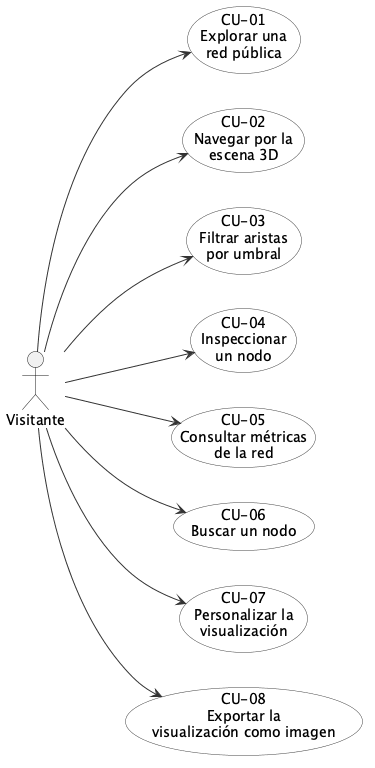
\includegraphics[height=14cm]{imagenes/cu_visitante}
	\caption{Diagrama de casos de uso del rol Visitante [V].}
	\label{fig:cu-visitante}
\end{figure}

\begin{figure}[H]
	\centering
	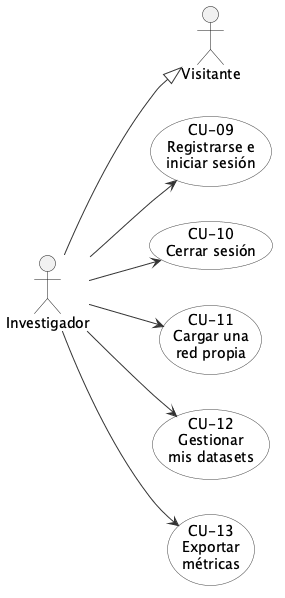
\includegraphics[height=12cm]{imagenes/cu_investigador}
	\caption{Diagrama de casos de uso del rol Investigador [I].}
	\label{fig:cu-investigador}
\end{figure}

\begin{figure}[H]
	\centering
	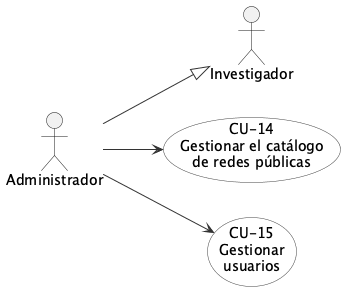
\includegraphics[height=6cm]{imagenes/cu_administrador}
	\caption{Diagrama de casos de uso del rol Administrador [A].}
	\label{fig:cu-administrador}
\end{figure}

\subsection{Descripción de los casos de uso}

Cada caso de uso se describe mediante una ficha detallada que recoge su actor, sus dependencias con
los requisitos funcionales, precondiciones, tipo, descripción, secuencia de pasos, postcondición y
excepciones (tablas~\ref{cu:01} a~\ref{cu:15}). Previamente, la tabla~\ref{tab:cu-resumen} muestra un
resumen con los casos de uso, su actor y los requisitos funcionales que implementan, poniendo de
manifiesto la trazabilidad entre requisitos y casos de uso.

\begin{table}[H]
	\centering
	\caption{Casos de uso y requisitos asociados.}
	\label{tab:cu-resumen}
	\small
	\begin{tabularx}{\textwidth}{>{\centering\arraybackslash}p{1.3cm} >{\raggedright\arraybackslash}X >{\raggedright\arraybackslash}p{2.5cm} >{\raggedright\arraybackslash}p{2.7cm}}
		\toprule
		\textbf{CU} & \textbf{Nombre} & \textbf{Actor} & \textbf{RF asociados} \\
		\midrule
		CU-01 & Explorar una red pública & Visitante & RF 2, RF 2.1 \\
		CU-02 & Navegar por la escena 3D & Visitante & RF 3 \\
		CU-03 & Filtrar aristas por umbral & Visitante & RF 5 \\
		CU-04 & Inspeccionar un nodo & Visitante & RF 6, RF 6.1 \\
		CU-05 & Consultar métricas de la red & Visitante & RF 8 \\
		CU-06 & Buscar un nodo & Visitante & RF 10 \\
		CU-07 & Personalizar la visualización & Visitante & RF 7, RF 9, RF 11 \\
		CU-08 & Exportar la visualización como imagen & Visitante & RF 12 \\
		\addlinespace
		CU-09 & Registrarse e iniciar sesión & Investigador & RF 13 \\
		CU-10 & Cerrar sesión & Investigador & RF 13 \\
		CU-11 & Cargar una red propia & Investigador & RF 14, RF 14.1 \\
		CU-12 & Gestionar mis conjuntos de datos & Investigador & RF 15 \\
		CU-13 & Exportar métricas & Investigador & RF 16 \\
		\addlinespace
		CU-14 & Gestionar el catálogo de redes públicas & Administrador & RF 17 \\
		CU-15 & Gestionar usuarios & Administrador & RF 18, RF 18.1 \\
		\bottomrule
	\end{tabularx}
\end{table}

% Fichas de casos de uso. Se usa xltabular para permitir el corte entre páginas.
% Columna 1: etiqueta del campo; Columna 2: contenido / acción.
\newcolumntype{K}{>{\raggedright\arraybackslash}p{3.3cm}}
\newcolumntype{V}{>{\raggedright\arraybackslash}X}
\setlength{\extrarowheight}{1.5pt}

% ------------------------------------------------------------------ CU-01
{\small
\begin{xltabular}{\textwidth}{|K|V|}
\caption{CU-01. Explorar una red pública.}\label{cu:01}\\
\hline
\rowcolor[gray]{0.88}\textbf{CU-01} & \textbf{Explorar una red pública} \\ \hline
\endfirsthead
\hline \rowcolor[gray]{0.88}\textbf{CU-01} & \textbf{Explorar una red pública (cont.)} \\ \hline
\endhead
\textbf{Actor principal} & Visitante [V] \\ \hline
\textbf{Dependencias} & RF 2, RF 2.1 \\ \hline
\textbf{Precondición} & La aplicación está desplegada y existe al menos una red pública disponible. \\ \hline
\textbf{Tipo} & Primario / Esencial \\ \hline
\textbf{Descripción} & El visitante selecciona una red pública y el sistema la procesa y la renderiza en 3D. \\ \hline
\rowcolor[gray]{0.88}\multicolumn{2}{|c|}{\textbf{Secuencia}} \\ \hline
\textbf{Paso} & \textbf{Acción} \\ \hline
1  & El visitante accede a la aplicación. \\ \hline
2  & El sistema muestra una red por defecto ya renderizado y la lista de redes disponibles. \\ \hline
3  & El visitante selecciona una red de la lista. \\ \hline
3a & El \textit{backend} procesa la red y la devuelve; el sistema la renderiza en 3D. \\ \hline
3b & La red no se puede cargar; se informa del error y se mantiene la anterior. \\ \hline
\textbf{Postcondición} & La red seleccionada queda visualizada en la escena 3D. \\ \hline
\textbf{Excepciones} & La red seleccionada no existe o está corrupto. \\ \hline
\textbf{Comentarios} & No aplica. \\ \hline
\end{xltabular}
}

% ------------------------------------------------------------------ CU-02
{\small
\begin{xltabular}{\textwidth}{|K|V|}
\caption{CU-02. Navegar por la escena 3D.}\label{cu:02}\\
\hline
\rowcolor[gray]{0.88}\textbf{CU-02} & \textbf{Navegar por la escena 3D} \\ \hline
\endfirsthead
\hline \rowcolor[gray]{0.88}\textbf{CU-02} & \textbf{Navegar por la escena 3D (cont.)} \\ \hline
\endhead
\textbf{Actor principal} & Visitante [V] \\ \hline
\textbf{Dependencias} & RF 3 \\ \hline
\textbf{Precondición} & Existe una red renderizada en la escena. \\ \hline
\textbf{Tipo} & Primario / Esencial \\ \hline
\textbf{Descripción} & El usuario explora la red rotando, haciendo zoom y desplazando la cámara. \\ \hline
\rowcolor[gray]{0.88}\multicolumn{2}{|c|}{\textbf{Secuencia}} \\ \hline
\textbf{Paso} & \textbf{Acción} \\ \hline
1 & El usuario arrastra, gira la rueda o desplaza sobre la escena. \\ \hline
2 & El sistema actualiza la cámara en tiempo real de forma fluida. \\ \hline
\textbf{Postcondición} & La vista de la cámara queda actualizada. \\ \hline
\textbf{Excepciones} & Fallo o falta de recursos gráficos en el dispositivo. \\ \hline
\textbf{Comentarios} & No aplica. \\ \hline
\end{xltabular}
}

% ------------------------------------------------------------------ CU-03
{\small
\begin{xltabular}{\textwidth}{|K|V|}
\caption{CU-03. Filtrar aristas por umbral.}\label{cu:03}\\
\hline
\rowcolor[gray]{0.88}\textbf{CU-03} & \textbf{Filtrar aristas por umbral} \\ \hline
\endfirsthead
\hline \rowcolor[gray]{0.88}\textbf{CU-03} & \textbf{Filtrar aristas por umbral (cont.)} \\ \hline
\endhead
\textbf{Actor principal} & Visitante [V] \\ \hline
\textbf{Dependencias} & RF 5 \\ \hline
\textbf{Precondición} & Existe una red renderizada con aristas ponderadas. \\ \hline
\textbf{Tipo} & Primario / Esencial \\ \hline
\textbf{Descripción} & El usuario ajusta un umbral y el sistema muestra solo las aristas con peso mayor o igual a él. \\ \hline
\rowcolor[gray]{0.88}\multicolumn{2}{|c|}{\textbf{Secuencia}} \\ \hline
\textbf{Paso} & \textbf{Acción} \\ \hline
1 & El usuario mueve el control deslizante de umbral. \\ \hline
2 & El sistema recalcula las aristas visibles y actualiza la escena y el contador. \\ \hline
\textbf{Postcondición} & Solo se muestran las aristas con peso por encima del umbral. \\ \hline
\textbf{Excepciones} & Ninguna. \\ \hline
\textbf{Comentarios} & Con el umbral en su valor mínimo se muestran todas las aristas de la red. \\ \hline
\end{xltabular}
}

% ------------------------------------------------------------------ CU-04
{\small
\begin{xltabular}{\textwidth}{|K|V|}
\caption{CU-04. Inspeccionar un nodo.}\label{cu:04}\\
\hline
\rowcolor[gray]{0.88}\textbf{CU-04} & \textbf{Inspeccionar un nodo} \\ \hline
\endfirsthead
\hline \rowcolor[gray]{0.88}\textbf{CU-04} & \textbf{Inspeccionar un nodo (cont.)} \\ \hline
\endhead
\textbf{Actor principal} & Visitante [V] \\ \hline
\textbf{Dependencias} & RF 6, RF 6.1 \\ \hline
\textbf{Precondición} & Existe una red renderizada. \\ \hline
\textbf{Tipo} & Primario / Esencial \\ \hline
\textbf{Descripción} & El usuario selecciona un nodo con un clic y consulta su información detallada y sus métricas de centralidad. \\ \hline
\rowcolor[gray]{0.88}\multicolumn{2}{|c|}{\textbf{Secuencia}} \\ \hline
\textbf{Paso} & \textbf{Acción} \\ \hline
1 & El usuario hace clic sobre un nodo. \\ \hline
2 & El sistema resalta el nodo y muestra su panel de información (etiqueta, coordenadas, grado, grupo y centralidades). \\ \hline
3 & El usuario hace clic en el espacio vacío para deseleccionar. \\ \hline
\textbf{Postcondición} & El nodo seleccionado queda resaltado y su información visible. \\ \hline
\textbf{Excepciones} & Ninguna. \\ \hline
\textbf{Comentarios} & Solo puede haber un nodo seleccionado a la vez. \\ \hline
\end{xltabular}
}

% ------------------------------------------------------------------ CU-05
{\small
\begin{xltabular}{\textwidth}{|K|V|}
\caption{CU-05. Consultar métricas de la red.}\label{cu:05}\\
\hline
\rowcolor[gray]{0.88}\textbf{CU-05} & \textbf{Consultar métricas de la red} \\ \hline
\endfirsthead
\hline \rowcolor[gray]{0.88}\textbf{CU-05} & \textbf{Consultar métricas de la red (cont.)} \\ \hline
\endhead
\textbf{Actor principal} & Visitante [V] \\ \hline
\textbf{Dependencias} & RF 8 \\ \hline
\textbf{Precondición} & Existe una red cargada en el sistema. \\ \hline
\textbf{Tipo} & Primario / Esencial \\ \hline
\textbf{Descripción} & El usuario consulta las métricas globales de la red calculadas en el \textit{backend}. \\ \hline
\rowcolor[gray]{0.88}\multicolumn{2}{|c|}{\textbf{Secuencia}} \\ \hline
\textbf{Paso} & \textbf{Acción} \\ \hline
1 & El usuario consulta el panel de métricas de la red. \\ \hline
2 & El sistema muestra densidad, grado medio, coeficiente de \textit{clustering} y componentes conexas. \\ \hline
\textbf{Postcondición} & Las métricas globales de la red quedan visibles. \\ \hline
\textbf{Excepciones} & Ninguna. \\ \hline
\textbf{Comentarios} & No aplica. \\ \hline
\end{xltabular}
}

% ------------------------------------------------------------------ CU-06
{\small
\begin{xltabular}{\textwidth}{|K|V|}
\caption{CU-06. Buscar un nodo.}\label{cu:06}\\
\hline
\rowcolor[gray]{0.88}\textbf{CU-06} & \textbf{Buscar un nodo} \\ \hline
\endfirsthead
\hline \rowcolor[gray]{0.88}\textbf{CU-06} & \textbf{Buscar un nodo (cont.)} \\ \hline
\endhead
\textbf{Actor principal} & Visitante [V] \\ \hline
\textbf{Dependencias} & RF 10 \\ \hline
\textbf{Precondición} & Existe una red renderizada. \\ \hline
\textbf{Tipo} & Secundario / Esencial \\ \hline
\textbf{Descripción} & El usuario busca un nodo por su etiqueta y la cámara se centra en él. \\ \hline
\rowcolor[gray]{0.88}\multicolumn{2}{|c|}{\textbf{Secuencia}} \\ \hline
\textbf{Paso} & \textbf{Acción} \\ \hline
1 & El usuario escribe un término en el campo de búsqueda. \\ \hline
2 & El sistema muestra las coincidencias por etiqueta. \\ \hline
3 & El usuario elige un resultado. \\ \hline
4 & El sistema resalta el nodo y centra la cámara sobre él. \\ \hline
\textbf{Postcondición} & La cámara queda centrada en el nodo encontrado. \\ \hline
\textbf{Excepciones} & No existen coincidencias para el término buscado. \\ \hline
\textbf{Comentarios} & No aplica. \\ \hline
\end{xltabular}
}

% ------------------------------------------------------------------ CU-07
{\small
\begin{xltabular}{\textwidth}{|K|V|}
\caption{CU-07. Personalizar la visualización.}\label{cu:07}\\
\hline
\rowcolor[gray]{0.88}\textbf{CU-07} & \textbf{Personalizar la visualización} \\ \hline
\endfirsthead
\hline \rowcolor[gray]{0.88}\textbf{CU-07} & \textbf{Personalizar la visualización (cont.)} \\ \hline
\endhead
\textbf{Actor principal} & Visitante [V] \\ \hline
\textbf{Dependencias} & RF 7, RF 9, RF 11 \\ \hline
\textbf{Precondición} & Existe una red renderizada. \\ \hline
\textbf{Tipo} & Secundario / Esencial \\ \hline
\textbf{Descripción} & El usuario ajusta el esquema de coloreado y tamaño de los nodos y otros parámetros visuales, y puede restablecer la vista. \\ \hline
\rowcolor[gray]{0.88}\multicolumn{2}{|c|}{\textbf{Secuencia}} \\ \hline
\textbf{Paso} & \textbf{Acción} \\ \hline
1  & El usuario ajusta el esquema de color/tamaño y los parámetros visuales. \\ \hline
2  & El sistema actualiza la escena de inmediato. \\ \hline
3a & (Flujo alternativo) El usuario pulsa ``restablecer'' y el sistema devuelve la vista a sus valores por defecto. \\ \hline
\textbf{Postcondición} & La escena refleja los ajustes elegidos por el usuario. \\ \hline
\textbf{Excepciones} & Ninguna. \\ \hline
\textbf{Comentarios} & El restablecimiento es un flujo alternativo, no un caso de uso independiente. \\ \hline
\end{xltabular}
}

% ------------------------------------------------------------------ CU-08
{\small
\begin{xltabular}{\textwidth}{|K|V|}
\caption{CU-08. Exportar la visualización como imagen.}\label{cu:08}\\
\hline
\rowcolor[gray]{0.88}\textbf{CU-08} & \textbf{Exportar la visualización como imagen} \\ \hline
\endfirsthead
\hline \rowcolor[gray]{0.88}\textbf{CU-08} & \textbf{Exportar la visualización como imagen (cont.)} \\ \hline
\endhead
\textbf{Actor principal} & Visitante [V] \\ \hline
\textbf{Dependencias} & RF 12 \\ \hline
\textbf{Precondición} & Existe una red renderizada en la escena. \\ \hline
\textbf{Tipo} & Secundario / Deseable \\ \hline
\textbf{Descripción} & El usuario exporta la vista actual de la escena 3D como una imagen PNG. \\ \hline
\rowcolor[gray]{0.88}\multicolumn{2}{|c|}{\textbf{Secuencia}} \\ \hline
\textbf{Paso} & \textbf{Acción} \\ \hline
1 & El usuario pulsa ``exportar imagen''. \\ \hline
2 & El sistema genera y descarga una imagen PNG de la escena. \\ \hline
\textbf{Postcondición} & Se descarga una imagen PNG con la vista actual. \\ \hline
\textbf{Excepciones} & Ninguna. \\ \hline
\textbf{Comentarios} & No aplica. \\ \hline
\end{xltabular}
}

% ------------------------------------------------------------------ CU-09
{\small
\begin{xltabular}{\textwidth}{|K|V|}
\caption{CU-09. Registrarse e iniciar sesión.}\label{cu:09}\\
\hline
\rowcolor[gray]{0.88}\textbf{CU-09} & \textbf{Registrarse e iniciar sesión} \\ \hline
\endfirsthead
\hline \rowcolor[gray]{0.88}\textbf{CU-09} & \textbf{Registrarse e iniciar sesión (cont.)} \\ \hline
\endhead
\textbf{Actor principal} & Investigador [I] \\ \hline
\textbf{Dependencias} & RF 13 \\ \hline
\textbf{Precondición} & El usuario se encuentra en la pantalla de acceso y no ha iniciado sesión previamente. \\ \hline
\textbf{Tipo} & Primario / Esencial \\ \hline
\textbf{Descripción} & El usuario se registra o inicia sesión para acceder a las funcionalidades de investigador. \\ \hline
\rowcolor[gray]{0.88}\multicolumn{2}{|c|}{\textbf{Secuencia}} \\ \hline
\textbf{Paso} & \textbf{Acción} \\ \hline
1  & El usuario abre el formulario de acceso. \\ \hline
2  & El sistema solicita las credenciales o el registro. \\ \hline
3  & El usuario introduce sus credenciales. \\ \hline
3a & Credenciales correctas: se inicia sesión con el rol investigador. \\ \hline
3b & Credenciales incorrectas: se informa y vuelve al paso 2. \\ \hline
\textbf{Postcondición} & El usuario accede a la aplicación con su rol y las funciones asociadas. \\ \hline
\textbf{Excepciones} & El usuario no está registrado; credenciales inválidas. \\ \hline
\textbf{Comentarios} & No aplica. \\ \hline
\end{xltabular}
}

% ------------------------------------------------------------------ CU-10
{\small
\begin{xltabular}{\textwidth}{|K|V|}
\caption{CU-10. Cerrar sesión.}\label{cu:10}\\
\hline
\rowcolor[gray]{0.88}\textbf{CU-10} & \textbf{Cerrar sesión} \\ \hline
\endfirsthead
\hline \rowcolor[gray]{0.88}\textbf{CU-10} & \textbf{Cerrar sesión (cont.)} \\ \hline
\endhead
\textbf{Actor principal} & Investigador [I] \\ \hline
\textbf{Dependencias} & RF 13 \\ \hline
\textbf{Precondición} & El usuario ha iniciado sesión previamente. \\ \hline
\textbf{Tipo} & Secundario / Esencial \\ \hline
\textbf{Descripción} & El usuario cierra su sesión y vuelve a actuar como visitante. \\ \hline
\rowcolor[gray]{0.88}\multicolumn{2}{|c|}{\textbf{Secuencia}} \\ \hline
\textbf{Paso} & \textbf{Acción} \\ \hline
1 & El usuario pulsa ``cerrar sesión''. \\ \hline
2 & El sistema finaliza la sesión y devuelve al usuario al estado no autenticado. \\ \hline
\textbf{Postcondición} & La sesión queda cerrada; el usuario pasa a actuar como visitante. \\ \hline
\textbf{Excepciones} & Ninguna. \\ \hline
\textbf{Comentarios} & Garantiza la seguridad al abandonar la aplicación, especialmente en equipos compartidos. \\ \hline
\end{xltabular}
}

% ------------------------------------------------------------------ CU-11
{\small
\begin{xltabular}{\textwidth}{|K|V|}
\caption{CU-11. Cargar una red propia.}\label{cu:11}\\
\hline
\rowcolor[gray]{0.88}\textbf{CU-11} & \textbf{Cargar una red propia} \\ \hline
\endfirsthead
\hline \rowcolor[gray]{0.88}\textbf{CU-11} & \textbf{Cargar una red propia (cont.)} \\ \hline
\endhead
\textbf{Actor principal} & Investigador [I] \\ \hline
\textbf{Dependencias} & RF 14, RF 14.1, RI 1, RI 2 \\ \hline
\textbf{Precondición} & El investigador se ha autenticado correctamente. \\ \hline
\textbf{Tipo} & Primario / Esencial \\ \hline
\textbf{Descripción} & El investigador sube sus ficheros \texttt{.node} y \texttt{.edge} para visualizar su propia red. \\ \hline
\rowcolor[gray]{0.88}\multicolumn{2}{|c|}{\textbf{Secuencia}} \\ \hline
\textbf{Paso} & \textbf{Acción} \\ \hline
1  & El investigador selecciona ``cargar red propia''. \\ \hline
2  & El sistema solicita los ficheros \texttt{.node} y \texttt{.edge}. \\ \hline
3  & El investigador sube ambos ficheros. \\ \hline
4  & El sistema valida el formato y la consistencia dimensional. \\ \hline
4a & Ficheros válidos: se procesa y se renderiza la red. \\ \hline
4b & Ficheros inválidos: se informa del error y vuelve al paso 2. \\ \hline
\textbf{Postcondición} & La red del investigador queda cargada y disponible para guardarse en sus \textit{conjuntos de datos}. \\ \hline
\textbf{Excepciones} & Dimensiones incongruentes entre ficheros; formato incorrecto; codificación inválida. \\ \hline
\textbf{Comentarios} & No aplica. \\ \hline
\end{xltabular}
}

% ------------------------------------------------------------------ CU-12
{\small
\begin{xltabular}{\textwidth}{|K|V|}
\caption{CU-12. Gestionar mis conjuntos de datos.}\label{cu:12}\\
\hline
\rowcolor[gray]{0.88}\textbf{CU-12} & \textbf{Gestionar mis conjuntos de datos} \\ \hline
\endfirsthead
\hline \rowcolor[gray]{0.88}\textbf{CU-12} & \textbf{Gestionar mis conjuntos de datos (cont.)} \\ \hline
\endhead
\textbf{Actor principal} & Investigador [I] \\ \hline
\textbf{Dependencias} & RF 15 \\ \hline
\textbf{Precondición} & El investigador se ha autenticado correctamente. \\ \hline
\textbf{Tipo} & Secundario / Esencial \\ \hline
\textbf{Descripción} & El investigador consulta, guarda, carga o elimina sus \textit{conjuntos de datos} privados. \\ \hline
\rowcolor[gray]{0.88}\multicolumn{2}{|c|}{\textbf{Secuencia}} \\ \hline
\textbf{Paso} & \textbf{Acción} \\ \hline
1  & El investigador abre la sección ``mis datasets''. \\ \hline
2  & El sistema muestra la lista de sus \textit{conjuntos de datos}. \\ \hline
3  & El investigador selecciona una acción. \\ \hline
3a & Guardar la red actual como un nuevo \textit{conjunto de datos}. \\ \hline
3b & Cargar un \textit{conjunto de datos} guardado para visualizarlo. \\ \hline
3c & Eliminar un \textit{conjunto de datos} existente. \\ \hline
4  & El sistema actualiza la lista de \textit{conjuntos de datos} del investigador. \\ \hline
\textbf{Postcondición} & La lista de \textit{conjuntos de datos} del investigador queda actualizada. \\ \hline
\textbf{Excepciones} & Ninguna. \\ \hline
\textbf{Comentarios} & Reúne las operaciones de guardar, listar, cargar y eliminar (CRUD) sobre los \textit{conjuntos de datos} propios. \\ \hline
\end{xltabular}
}

% ------------------------------------------------------------------ CU-13
{\small
\begin{xltabular}{\textwidth}{|K|V|}
\caption{CU-13. Exportar métricas.}\label{cu:13}\\
\hline
\rowcolor[gray]{0.88}\textbf{CU-13} & \textbf{Exportar métricas} \\ \hline
\endfirsthead
\hline \rowcolor[gray]{0.88}\textbf{CU-13} & \textbf{Exportar métricas (cont.)} \\ \hline
\endhead
\textbf{Actor principal} & Investigador [I] \\ \hline
\textbf{Dependencias} & RF 16 \\ \hline
\textbf{Precondición} & El investigador está autenticado y hay una red con métricas calculadas. \\ \hline
\textbf{Tipo} & Secundario / Esencial \\ \hline
\textbf{Descripción} & El investigador exporta las métricas de la red en formato CSV o JSON. \\ \hline
\rowcolor[gray]{0.88}\multicolumn{2}{|c|}{\textbf{Secuencia}} \\ \hline
\textbf{Paso} & \textbf{Acción} \\ \hline
1 & El investigador pulsa ``exportar métricas''. \\ \hline
2 & El sistema solicita el formato (CSV o JSON). \\ \hline
3 & El investigador elige el formato. \\ \hline
4 & El sistema genera y descarga el fichero de métricas. \\ \hline
\textbf{Postcondición} & Se descarga el fichero de métricas en el formato elegido. \\ \hline
\textbf{Excepciones} & Ninguna. \\ \hline
\textbf{Comentarios} & No aplica. \\ \hline
\end{xltabular}
}

% ------------------------------------------------------------------ CU-14
{\small
\begin{xltabular}{\textwidth}{|K|V|}
\caption{CU-14. Gestionar el catálogo de redes públicas.}\label{cu:14}\\
\hline
\rowcolor[gray]{0.88}\textbf{CU-14} & \textbf{Gestionar el catálogo de redes públicas} \\ \hline
\endfirsthead
\hline \rowcolor[gray]{0.88}\textbf{CU-14} & \textbf{Gestionar el catálogo de redes públicas (cont.)} \\ \hline
\endhead
\textbf{Actor principal} & Administrador [A] \\ \hline
\textbf{Dependencias} & RF 17 \\ \hline
\textbf{Precondición} & El administrador se ha autenticado correctamente. \\ \hline
\textbf{Tipo} & Primario / Esencial \\ \hline
\textbf{Descripción} & El administrador añade, edita o elimina las redes públicas disponibles para todos los usuarios. \\ \hline
\rowcolor[gray]{0.88}\multicolumn{2}{|c|}{\textbf{Secuencia}} \\ \hline
\textbf{Paso} & \textbf{Acción} \\ \hline
1  & El administrador abre la gestión del catálogo. \\ \hline
2  & El sistema muestra las redes públicas actuales. \\ \hline
3  & El administrador selecciona una acción. \\ \hline
3a & Añadir una red subiendo sus ficheros. \\ \hline
3b & Editar los metadatos de una red existente. \\ \hline
3c & Eliminar una red existente. \\ \hline
4  & El sistema valida los datos y actualiza el catálogo público. \\ \hline
\textbf{Postcondición} & El catálogo de redes públicas queda actualizado para todos los usuarios. \\ \hline
\textbf{Excepciones} & Ficheros de la red inválidos; la red ya está registrada. \\ \hline
\textbf{Comentarios} & Reúne las operaciones de añadir, editar y eliminar (CRUD) sobre el catálogo público. \\ \hline
\end{xltabular}
}

% ------------------------------------------------------------------ CU-15
{\small
\begin{xltabular}{\textwidth}{|K|V|}
\caption{CU-15. Gestionar usuarios.}\label{cu:15}\\
\hline
\rowcolor[gray]{0.88}\textbf{CU-15} & \textbf{Gestionar usuarios} \\ \hline
\endfirsthead
\hline \rowcolor[gray]{0.88}\textbf{CU-15} & \textbf{Gestionar usuarios (cont.)} \\ \hline
\endhead
\textbf{Actor principal} & Administrador [A] \\ \hline
\textbf{Dependencias} & RF 18, RF 18.1 \\ \hline
\textbf{Precondición} & El administrador se ha autenticado correctamente. \\ \hline
\textbf{Tipo} & Primario / Esencial \\ \hline
\textbf{Descripción} & El administrador consulta los usuarios, cambia su rol o los elimina. \\ \hline
\rowcolor[gray]{0.88}\multicolumn{2}{|c|}{\textbf{Secuencia}} \\ \hline
\textbf{Paso} & \textbf{Acción} \\ \hline
1  & El administrador abre la gestión de usuarios. \\ \hline
2  & El sistema muestra la lista de usuarios y sus roles. \\ \hline
3  & El administrador selecciona una acción. \\ \hline
3a & Asignar o revocar el rol de investigador a un usuario. \\ \hline
3b & Eliminar un usuario. \\ \hline
4  & El sistema actualiza los usuarios y sus roles. \\ \hline
\textbf{Postcondición} & Los usuarios y sus roles quedan actualizados correctamente. \\ \hline
\textbf{Excepciones} & Ninguna. \\ \hline
\textbf{Comentarios} & Reúne las operaciones de listar, editar el rol y eliminar usuarios. \\ \hline
\end{xltabular}
}


\section{Asignación de requisitos a los sprints y criterios de validación}

Antes de abordar la validación conviene fijar en qué sprint se implementará cada requisito. La
tabla~\ref{tab:validacion} muestra la asignación de los requisitos a cada uno de los sprints del
proyecto, junto con las pruebas de validación previstas para cada uno. Esta asignación sigue el orden
de prioridad establecido en la tabla~\ref{tab:priorizacion}.

La validación de la aplicación se llevará a cabo considerando el grado de cumplimiento de los
requisitos funcionales, no funcionales y de información, así como la implementación directa de los
distintos casos de uso. A lo largo del desarrollo se realizarán pruebas de software al finalizar cada
parte desarrollada, que abarcarán desde pruebas unitarias y de integración, destinadas a verificar el
funcionamiento del código, hasta pruebas de validación que aseguren el cumplimiento de los
requisitos. Además, al finalizar cada sprint se realizará una validación por parte del cliente ---en
este caso, el director del proyecto---, para lo cual la aplicación se desplegará en un servidor
accesible.

\begin{table}[H]
	\centering
	\caption{Asignación de requisitos a los sprints y pruebas de validación.}
	\label{tab:validacion}
	\begin{tabularx}{\textwidth}{>{\centering\arraybackslash}p{1.4cm} >{\raggedright\arraybackslash}p{3.2cm} >{\raggedright\arraybackslash}X}
		\toprule
		\textbf{Sprint} & \textbf{Requisitos} & \textbf{Pruebas de validación} \\
		\midrule
		1 & RF 1 -- RF 4 &
			Carga de una red pública; renderizado 3D correcto; navegación fluida [RNF 1]; el HUD
			muestra las cifras de la red. \\
		\addlinespace
		2 & RF 5 -- RF 7 &
			El control deslizante filtra aristas y el contador se actualiza; el clic selecciona un
			nodo y muestra su información; coloreado por grupo con leyenda. \\
		\addlinespace
		3 & RF 6.1, RF 8 -- RF 10 &
			Métricas globales y por nodo correctas (contraste manual con una implementación de
			referencia); mapeo visual por métrica; la búsqueda centra la cámara en el nodo. \\
		\addlinespace
		4 & RF 11 -- RF 18 &
			Registro e inicio de sesión; subida y validación de ficheros; gestión de conjuntos de
			datos; confidencialidad de datos privados [RNF 2]; gestión de catálogo y usuarios por el
			administrador; exportación. \\
		\bottomrule
	\end{tabularx}
\end{table}

La planificación temporal de cada sprint, así como los recursos y el coste asociados, se describen en
el capítulo correspondiente.


	% Cap. 3 - Plan del proyecto
	%   3.1 Recursos (humanos, materiales)
	%   3.2 Planificación temporal
	%   3.3 Análisis de tecnologías disponibles
	%   3.4 Estimación de costes
	\chapter{Plan del proyecto}

Una vez definidos los requisitos del sistema, es necesario establecer una estrategia de ejecución
detallada antes de la fase de desarrollo. El objetivo de este capítulo es fijar los recursos
necesarios, organizar las tareas en el tiempo mediante una planificación en forma de calendario,
analizar las tecnologías elegidas para cada componente y calcular el coste final estimado del
proyecto.

El desarrollo se estructura de forma ágil, basada en \textit{sprints} (ciclos cortos de trabajo),
con el objetivo de ir creando pequeñas versiones funcionales del proyecto de manera continua. Esto
aumenta la claridad del desarrollo y la capacidad de adaptación ante cambios o errores detectados a
lo largo del proceso, y permite al director validar los avances \textit{sprint} a \textit{sprint}.

\section{Recursos}

Es fundamental establecer con qué medios se cuenta para realizar el proyecto. Se dividen en dos
grupos: los recursos humanos y los recursos materiales. Como es lógico en un TFG, el alumno asume
todos los roles, pero para poder hacer una estimación realista de costes se toma como referencia el
mercado laboral actual de España, simulando que el proyecto lo llevan a cabo varios profesionales.

\subsection{Recursos humanos}

Dependiendo de la fase del proyecto en la que se esté, hace falta un perfil técnico u otro. Teniendo
esto en cuenta, se han definido los cinco roles que recoge la tabla~\ref{tab:salarios}, con una
estimación de su salario medio.

\begin{table}[H]
	\centering
	\caption{Salario medio del personal.}
	\label{tab:salarios}
	\begin{tabularx}{0.75\textwidth}{X r r}
		\toprule
		\textbf{Rol} & \textbf{Salario anual bruto} & \textbf{Salario por hora} \\
		\midrule
		Analista                  & 31.500\,\euro{} & 16,15\,\euro{} \\
		Ingeniero de Datos        & 30.000\,\euro{} & 15,38\,\euro{} \\
		Ingeniero de Requisitos   & 35.000\,\euro{} & 17,95\,\euro{} \\
		Ingeniero de Software     & 35.000\,\euro{} & 17,95\,\euro{} \\
		Programador               & 28.500\,\euro{} & 14,62\,\euro{} \\
		\bottomrule
	\end{tabularx}
\end{table}

Estos datos son una aproximación basada en ofertas reales del sector~\cite{salarios}, y pueden variar
en función del momento en el que se consulten o del nivel y experiencia de los profesionales. Estos
cinco roles intervienen en distintas fases del proyecto: en las fases iniciales de ingeniería
participan el Analista y el Ingeniero de Requisitos, mientras que en los sprints de desarrollo lo
hacen el Ingeniero de Datos, el Ingeniero de Software y el Programador. Al ser Brain Viz una
aplicación web de visualización 3D, dentro de cada sprint las tareas se dividen entre \textit{backend}
y \textit{frontend}, tal y como resume la tabla~\ref{tab:secciones}.

\begin{table}[H]
	\centering
	\caption{Secciones típicas dentro de un sprint de desarrollo y rol encargado.}
	\label{tab:secciones}
	\begin{tabularx}{\textwidth}{X >{\centering\arraybackslash}p{1.8cm} l}
		\toprule
		\textbf{Sección} & \textbf{Capa} & \textbf{Encargado} \\
		\midrule
		Procesamiento de datos y algoritmos        & Backend  & Ingeniero de Datos \\
		Diseñar la API y su comunicación           & Backend  & Ingeniero de Software \\
		Diseñar el entorno y la visualización 3D   & Frontend & Ingeniero de Software \\
		Programación e integración del código      & Ambas    & Programador \\
		Pruebas de software y validación           & Ambas    & Ingeniero de Software \\
		\bottomrule
	\end{tabularx}
\end{table}

\subsection{Recursos materiales}

Para sacar adelante la aplicación también es fundamental contar con las herramientas adecuadas,
además del personal técnico. Para estimar el coste del software y del hardware se toma como
referencia lo que marca la Ley del Impuesto sobre Sociedades, que permite estimar una vida útil de 6
años (2190 días) para los productos software y de 8 años (2920 días) para el hardware; el coste
diario es la parte proporcional (amortización) que corresponde al periodo de uso del proyecto. Las
tablas~\ref{tab:software} y~\ref{tab:hardware} recogen, respectivamente, los productos software y
hardware utilizados. Una ventaja importante es que la mayoría de las tecnologías empleadas en el
desarrollo (Docker, Python, Flask, NetworkX, React, Three.js o VS~Code, entre otras) son
\textbf{gratuitas o de código abierto}, por lo que no suponen coste alguno.

\begin{table}[H]
	\centering
	\caption{Productos software utilizados.}
	\label{tab:software}
	\begin{tabularx}{\textwidth}{X r c r}
		\toprule
		\textbf{Licencias} & \textbf{Coste total} & \textbf{Amortización} & \textbf{Coste diario} \\
		\midrule
		Microsoft Windows 11 Pro               & 145,00\,\euro{} & 2190 días & 0,066\,\euro{}/día \\
		Microsoft Office 2024                   & 299,00\,\euro{} & 2190 días & 0,137\,\euro{}/día \\
		VS Code y otras tecnologías gratuitas  & 0,00\,\euro{}   & 2190 días & 0,000\,\euro{}/día \\
		\midrule
		\multicolumn{3}{r}{\textbf{Total}} & \textbf{0,203\,\euro{}/día} \\
		\bottomrule
	\end{tabularx}
\end{table}

\begin{table}[H]
	\centering
	\caption{Productos hardware utilizados.}
	\label{tab:hardware}
	\begin{tabularx}{\textwidth}{X l r c r}
		\toprule
		\textbf{Producto} & \textbf{Tipo} & \textbf{Coste total} & \textbf{Amortización} & \textbf{Coste diario} \\
		\midrule
		ASUS Zenbook 14         & Portátil & 1.099,00\,\euro{} & 2920 días & 0,38\,\euro{}/día \\
		HP OMEN 24 180Hz        & Monitor  & 169,00\,\euro{}   & 2920 días & 0,06\,\euro{}/día \\
		Logitech G203           & Ratón    & 29,99\,\euro{}    & 2920 días & 0,01\,\euro{}/día \\
		Teclado inalámbrico TKL & Teclado  & 69,99\,\euro{}    & 2920 días & 0,02\,\euro{}/día \\
		\midrule
		\multicolumn{4}{r}{\textbf{Total}} & \textbf{0,47\,\euro{}/día} \\
		\bottomrule
	\end{tabularx}
\end{table}

Además de los equipos, el proyecto requiere \textbf{desplegar la aplicación en un servidor público}
para que el director pueda validar cada sprint y, más adelante, el tribunal pueda probarla con
facilidad. Para ello se contempla un servidor virtual (VPS) de bajo coste, estimado en
6,00\,\euro{}/mes.

\section{Planificación temporal}

Para organizar la planificación en forma de calendario se toman jornadas laborales estándar de 8
horas. El desarrollo se divide en cuatro \textit{sprints}, que se corresponden con los cuatro niveles
de prioridad de los requisitos funcionales definidos en el capítulo de requisitos; la asignación
concreta de requisitos a cada sprint se detalló en la tabla~\ref{tab:validacion} de dicho capítulo.
La tabla~\ref{tab:estimacion-sprint} muestra la estimación de días laborables que llevará completar
cada sprint.

\begin{table}[H]
	\centering
	\caption{Estimación temporal por sprint.}
	\label{tab:estimacion-sprint}
	\begin{tabularx}{0.7\textwidth}{>{\centering\arraybackslash}X >{\centering\arraybackslash}X}
		\toprule
		\textbf{Sprint} & \textbf{Estimación temporal} \\
		\midrule
		Sprint 1 & 8 días \\
		Sprint 2 & 7 días \\
		Sprint 3 & 7 días \\
		Sprint 4 & 5 días \\
		\bottomrule
	\end{tabularx}
\end{table}

Además del desarrollo de los \textit{sprints}, el proyecto incluye tareas previas de ingeniería
(análisis de requisitos, casos de uso, planificación y estudio de tecnologías) y la redacción de la
memoria, que se realiza en paralelo al desarrollo y a la que se dedican además algunos días finales
para rematarla y preparar la presentación. La tabla~\ref{tab:tareas} enumera todas las tareas del
proyecto con su responsable y su estimación temporal, e incluye una fila final con el total de días
de trabajo.

\begin{table}[H]
	\centering
	\caption{Tareas del proyecto y estimación temporal.}
	\label{tab:tareas}
	\begin{tabularx}{\textwidth}{>{\centering\arraybackslash}p{1cm} >{\raggedright\arraybackslash}X >{\raggedright\arraybackslash}p{4.2cm} >{\centering\arraybackslash}p{2.1cm}}
		\toprule
		\textbf{N.º} & \textbf{Tarea} & \textbf{Encargado} & \textbf{Estimación} \\
		\midrule
		1 & Análisis de requisitos       & Ingeniero de Requisitos & 3 días \\
		2 & Análisis de casos de uso     & Ingeniero de Requisitos & 2 días \\
		3 & Planificación del proyecto   & Analista                & 2 días \\
		4 & Estudio de tecnologías       & Analista                & 2 días \\
		5 & Sprint 1                     & Equipo de desarrollo    & 8 días \\
		6 & Sprint 2                     & Equipo de desarrollo    & 7 días \\
		7 & Sprint 3                     & Equipo de desarrollo    & 7 días \\
		8 & Sprint 4                     & Equipo de desarrollo    & 5 días \\
		9 & Redacción de la memoria y preparación de la presentación & Analista & 2 días \\
		\midrule
		\multicolumn{3}{r}{\textbf{Total}} & \textbf{38 días} \\
		\bottomrule
	\end{tabularx}
\end{table}

La estimación total (38 días laborables, unas 300 horas) es coherente con la carga de trabajo
esperada para un Trabajo Fin de Grado de 12 créditos ECTS. La redacción de la memoria se lleva a cabo
mayoritariamente en paralelo al desarrollo, reservando los días finales para rematarla y preparar la
defensa. Para representar gráficamente el cronograma y las dependencias entre tareas se utiliza el
diagrama de Gantt de la figura~\ref{fig:gantt}, en el que se aprecian las tareas iniciales de
ingeniería, los cuatro \textit{sprints} de desarrollo encadenados y la redacción de la memoria en
paralelo al desarrollo. Para no ligar el cronograma a fechas concretas ---que no encajarían con un
TFG que puede defenderse en distintas convocatorias--- se emplean meses genéricos (mes~1, mes~2,
etc.).

\begin{figure}[H]
	\centering
	\begin{tikzpicture}[font=\small]
		% --- Parámetros: x(d) = 4.4 + 0.24*d (d en días laborables) ---
		% Bandas de meses (cada mes ~20 días laborables)
		\fill[blue!6]  (4.4,0.75) rectangle (9.2,6.35);
		\fill[green!6] (9.2,0.75) rectangle (14.0,6.35);
		\node at (6.8,6.05) {\bfseries Mes 1};
		\node at (11.6,6.05) {\bfseries Mes 2};
		% Separadores verticales de mes
		\foreach \x in {4.4,9.2,14.0} \draw[gray!50] (\x,0.75) -- (\x,5.75);
		% Líneas de rejilla por semana (cada 5 días)
		\foreach \d in {5,10,15,25,30,35} \draw[gray!20] ({4.4+0.24*\d},0.85) -- ({4.4+0.24*\d},5.7);

		% --- Filas (etiquetas) ---
		\foreach \y/\name in {%
			5.50/Análisis de requisitos,
			4.95/Casos de uso,
			4.40/Planificación del proyecto,
			3.85/Estudio de tecnologías,
			3.30/Sprint 1,
			2.75/Sprint 2,
			2.20/Sprint 3,
			1.65/Sprint 4,
			1.10/Memoria y presentación}
			\node[anchor=east] at (4.2,\y) {\name};

		% --- Barras: \fill de x(inicio) a x(fin) ---
		\definecolor{ging}{RGB}{120,160,220}
		\definecolor{gdev}{RGB}{120,195,140}
		\definecolor{gmem}{RGB}{235,190,120}
		\tikzset{bar/.style={rounded corners=1.5pt, draw=black!30}}
		\fill[bar,fill=ging] (4.40,5.32) rectangle (5.12,5.68); % 0-3
		\fill[bar,fill=ging] (5.12,4.77) rectangle (5.60,5.13); % 3-5
		\fill[bar,fill=ging] (5.60,4.22) rectangle (6.08,4.58); % 5-7
		\fill[bar,fill=ging] (6.08,3.67) rectangle (6.56,4.03); % 7-9
		\fill[bar,fill=gdev] (6.56,3.12) rectangle (8.48,3.48); % 9-17
		\fill[bar,fill=gdev] (8.48,2.57) rectangle (10.16,2.93); % 17-24
		\fill[bar,fill=gdev] (10.16,2.02) rectangle (11.84,2.38); % 24-31
		\fill[bar,fill=gdev] (11.84,1.47) rectangle (13.04,1.83); % 31-36
		\fill[bar,fill=gmem] (6.56,0.92) rectangle (13.52,1.28); % 9-38 (paralelo)

		% --- Leyenda ---
		\fill[bar,fill=ging] (4.4,0.25) rectangle (4.75,0.5); \node[anchor=west] at (4.8,0.375) {Ingeniería};
		\fill[bar,fill=gdev] (7.1,0.25) rectangle (7.45,0.5); \node[anchor=west] at (7.5,0.375) {Desarrollo (sprints)};
		\fill[bar,fill=gmem] (10.8,0.25) rectangle (11.15,0.5); \node[anchor=west] at (11.2,0.375) {Memoria};
	\end{tikzpicture}
	\caption{Diagrama de Gantt del proyecto (meses genéricos).}
	\label{fig:gantt}
\end{figure}

\section{Análisis de tecnologías disponibles}

La aplicación se divide en dos componentes principales: un \textbf{servicio de backend}, encargado
del procesamiento y análisis de las redes y de exponer los resultados a través de una API, y una
\textbf{aplicación cliente o frontend}, encargada de la interacción con el usuario y de la
visualización 3D en el navegador. Este es el punto del proyecto en el que se decide qué tecnologías
se van a utilizar; por eso en los capítulos anteriores se ha evitado citar tecnologías concretas. La
selección se ha basado en la idoneidad para el problema específico. A continuación se analizan y
comparan las tecnologías consideradas.

\subsection{Framework de backend y análisis de grafos}

El backend debe servir los datos de las redes al cliente a través de una API y utilizar bibliotecas
de análisis de grafos para el procesamiento de las matrices de adyacencia. Dado que Python dispone de
bibliotecas de análisis de grafos nativas (NetworkX~\cite{networkx}, igraph~\cite{igraph} o
graph-tool~\cite{graphtool}), elegir un \textit{framework} de backend en Python es la decisión más
eficiente, evitando la dificultad de crear servicios de intercomunicación entre lenguajes. La
tabla~\ref{tab:backend} compara las alternativas de \textit{framework} de backend consideradas.

\begin{table}[H]
	\centering
	\caption{Alternativas de backend en Python.}
	\label{tab:backend}
	\small
	\begin{tabularx}{\textwidth}{>{\raggedright\arraybackslash}p{2.0cm} >{\raggedright\arraybackslash}p{3.1cm} >{\raggedright\arraybackslash}X}
		\toprule
		\textbf{Framework} & \textbf{Arquitectura} & \textbf{Utilidad para el proyecto} \\
		\midrule
		Django & Monolítico (Full-stack, ``pilas incluidas'') &
			Incluye un ORM (mapeo objeto-relacional), un panel de administrador y un sistema de
			autenticación. Estos elementos no son imprescindibles para el núcleo de Brain Viz, el cual
			se enfoca en un servicio de datos. \\
		\addlinespace
		Flask & Micro-framework (Minimalista) &
			Para desarrollar APIs REST livianas, Flask es perfecto. Posibilita una integración simple y
			directa con librerías como NetworkX. Su filosofía minimalista posibilita construir
			únicamente lo que se necesita, lo cual es ideal para un servicio de API limitado. \\
		\addlinespace
		FastAPI & Micro-framework (Moderno, Asíncrono) &
			Proporciona un rendimiento más elevado debido a su carácter asíncrono (ASGI). Produce de
			manera automática documentación interactiva (OpenAPI/Swagger), lo que representa un beneficio
			importante para el desarrollo y la depuración de la API. \\
		\bottomrule
	\end{tabularx}
\end{table}

\textbf{Selección final:} se descarta Django por su enfoque monolítico, innecesario aquí. Entre Flask
y FastAPI se elige \textbf{Flask}~\cite{flask}, ya que permite crear una API totalmente funcional para
leer los ficheros de forma directa, procesarlos con NetworkX~\cite{networkx} y enviarlos como JSON al
frontend con la máxima sencillez.

\subsection{Framework de frontend (UI)}

El frontend es la parte con la que interactúa el usuario. Debe gestionar la visualización 3D y
controlar el estado de la aplicación. La tabla~\ref{tab:frontend} compara las alternativas
consideradas.

\begin{table}[H]
	\centering
	\caption{Alternativas de frontend.}
	\label{tab:frontend}
	\small
	\begin{tabularx}{\textwidth}{>{\raggedright\arraybackslash}p{1.9cm} >{\raggedright\arraybackslash}p{3.1cm} >{\raggedright\arraybackslash}p{3.1cm} >{\raggedright\arraybackslash}X}
		\toprule
		\textbf{Framework} & \textbf{Paradigma} & \textbf{Ecosistema} & \textbf{Integración 3D} \\
		\midrule
		React & Basado en componentes (Declarativo) &
			Enorme. Mantenido por Meta. &
			Contiene bindings que integran Three.js. \\
		\addlinespace
		Vue.js & Basado en componentes (Progresivo) &
			Grande. Impulsado por la comunidad. &
			Existen integraciones como \textit{trois}, que también integran Three.js. \\
		\addlinespace
		Angular & Framework completo (MVC, Modelo-Vista-Controlador) &
			Grande. Mantenido por Google. &
			La integración con librerías 3D es menos común o de más bajo nivel. \\
		\bottomrule
	\end{tabularx}
\end{table}

\textbf{Selección final:} se elige \textbf{React}~\cite{react}. Se descarta Angular por su rigidez, y
frente a Vue, React ofrece una ventaja decisiva gracias a su ecosistema de visualización 3D, en
concreto al \textit{binding} \textit{react-three-fiber}~\cite{r3f}, que permite desarrollar con gran
potencia el renderizado 3D usando Three.js.

\subsection{Tecnología de visualización 3D}

Para renderizar contenido 3D en el navegador existen distintas posibilidades a bajo nivel: el
elemento \textit{canvas} 2D (insuficiente para 3D acelerado), \textbf{WebGL}~\cite{webgl} ---el
estándar actual para el renderizado 3D acelerado por hardware en el navegador--- y el más reciente
\textbf{WebGPU}~\cite{webgpu}, todavía en adopción y con soporte desigual entre navegadores. Por su
madurez y compatibilidad, se opta por una solución basada en WebGL. Sobre esta base, la biblioteca de
alto nivel elegida debe ser capaz de renderizar grafos y permitir una interacción fluida para una
buena experiencia de usuario. La tabla~\ref{tab:viz3d} compara las bibliotecas y motores considerados.

\begin{table}[H]
	\centering
	\caption{Tecnologías de visualización 3D consideradas.}
	\label{tab:viz3d}
	\small
	\begin{tabularx}{\textwidth}{>{\raggedright\arraybackslash}p{2.4cm} >{\raggedright\arraybackslash}p{2.3cm} >{\raggedright\arraybackslash}p{1.7cm} >{\raggedright\arraybackslash}X}
		\toprule
		\textbf{Tecnología} & \textbf{Tipo} & \textbf{Nivel de abstracción} & \textbf{Caso de uso} \\
		\midrule
		PlayCanvas~\cite{playcanvas} & Motor de juego 3D (con editor) & Alto &
			Motor enfocado al desarrollo de videojuegos, con editor visual en la nube, pero su modelo no
			se adapta a la carga dinámica de datos. \\
		\addlinespace
		luma.gl / deck.gl~\cite{lumagl} & Framework de visualización de datos & Alto (geodatos) &
			Optimizado para la carga y visualización de grandes cantidades de datos geoespaciales, como
			mapas. No diseñado para grafos abstractos en 3D. \\
		\addlinespace
		graph.gl~\cite{graphgl} & Framework de visualización de grafos & Alto (grafos) &
			Proyecto con una comunidad pequeña y menos mantenido que el resto de alternativas. Alto
			riesgo de encontrar problemas y poca documentación. \\
		\addlinespace
		Babylon.js~\cite{babylon} & Motor de juego / framework 3D & Medio-Alto &
			Mantenido por Microsoft. Es un ``todo en uno'' muy potente y relativamente sencillo.
			Ecosistema robusto. \\
		\addlinespace
		Three.js~\cite{threejs} & Librería de renderizado 3D & Bajo &
			Es el estándar en la industria. La librería WebGL de más bajo nivel y más utilizada. Requiere
			más esfuerzo en la gestión de escena, cámaras, luces y bucle de renderizado manual. \\
		\bottomrule
	\end{tabularx}
\end{table}

\textbf{Selección final:} se descartan PlayCanvas, luma.gl y graph.gl por no ajustarse al uso de
visualización de datos 3D. La elección se encuentra entre Babylon.js y Three.js; ligada a la elección
previa de React, lo más lógico es
usar \textbf{Three.js~\cite{threejs} mediante \textit{react-three-fiber}}. Esta combinación aporta la
potencia y flexibilidad de Three.js con la facilidad de uso de React, ya que permite declarar
componentes como luces o cámaras igual que componentes de React, eliminando las dificultades del
bucle de renderizado manual y facilitando la conexión con el estado de la aplicación.

\subsection{Resumen del stack seleccionado}

La tabla~\ref{tab:stack} resume el stack tecnológico finalmente seleccionado para cada componente del
sistema.

\begin{table}[H]
	\centering
	\caption{Resumen del stack tecnológico seleccionado.}
	\label{tab:stack}
	\small
	\begin{tabularx}{\textwidth}{>{\raggedright\arraybackslash}p{2.2cm} >{\raggedright\arraybackslash}p{2.3cm} >{\raggedright\arraybackslash}p{2.9cm} >{\raggedright\arraybackslash}X}
		\toprule
		\textbf{Componente} & \textbf{Tecnología principal} & \textbf{Bibliotecas} & \textbf{Justificación} \\
		\midrule
		Backend & Python & Flask, NetworkX &
			Integración nativa para análisis de grafos, eficiencia y enfoque minimalista para APIs REST. \\
		\addlinespace
		Frontend & JavaScript & React, Three.js, react-three-fiber &
			Modelo declarativo de componentes, ecosistema líder y la mejor integración de su clase entre
			UI y renderizado 3D. \\
		\addlinespace
		Despliegue & Docker & Docker, Docker Compose &
			Garantiza la reproducibilidad del entorno y facilita la orquestación de los servicios de
			backend y frontend. \\
		\bottomrule
	\end{tabularx}
\end{table}

\section{Estimación de costes}

Para cerrar el capítulo se recopilan todos los datos calculados y se presenta la estimación de costes
final. El esfuerzo en recursos humanos se obtiene sumando, para cada tarea, el número de horas por el
salario por hora del rol encargado, tal y como detalla la tabla~\ref{tab:coste-humano}. El proyecto
tiene una duración total de 38 días laborables (unas 300 horas), periodo utilizado también para
calcular la parte proporcional de amortización de los equipos y las licencias.

\begin{table}[H]
	\centering
	\caption{Coste de los recursos humanos por tarea.}
	\label{tab:coste-humano}
	\small
	\begin{tabularx}{\textwidth}{>{\raggedright\arraybackslash}X >{\raggedright\arraybackslash}p{3.2cm} >{\centering\arraybackslash}p{1.1cm} >{\centering\arraybackslash}p{1.2cm} r}
		\toprule
		\textbf{Tarea} & \textbf{Rol} & \textbf{Días} & \textbf{Horas} & \textbf{Coste} \\
		\midrule
		Análisis de requisitos & Ingeniero de Requisitos & 3 & 24 & 430,80\,\euro{} \\
		Análisis de casos de uso & Ingeniero de Requisitos & 2 & 16 & 287,20\,\euro{} \\
		Planificación del proyecto & Analista & 2 & 16 & 258,40\,\euro{} \\
		Estudio de tecnologías & Analista & 2 & 16 & 258,40\,\euro{} \\
		Sprint 1 & Ingeniero de Software & 8 & 64 & 1.148,80\,\euro{} \\
		Sprint 2 & Programador & 7 & 56 & 818,72\,\euro{} \\
		Sprint 3 & Ingeniero de Datos & 7 & 56 & 861,28\,\euro{} \\
		Sprint 4 & Programador & 5 & 40 & 584,80\,\euro{} \\
		Redacción memoria y presentación & Analista & 2 & 16 & 258,40\,\euro{} \\
		\midrule
		\textbf{Total} & & \textbf{38} & \textbf{304} & \textbf{4.906,80\,\euro{}} \\
		\bottomrule
	\end{tabularx}
\end{table}

A este coste de personal se suman la amortización de los equipos y las licencias durante los 38 días
del proyecto y el coste de desplegar la aplicación en un servidor público durante el periodo de
validación y defensa (estimado en 6 meses). La tabla~\ref{tab:coste-total} recoge la estimación final.

\begin{table}[H]
	\centering
	\caption{Estimación de costes total del proyecto.}
	\label{tab:coste-total}
	\begin{tabularx}{0.9\textwidth}{X r}
		\toprule
		\textbf{Recursos} & \textbf{Coste} \\
		\midrule
		Recursos humanos                                         & 4.906,80\,\euro{} \\
		Recursos hardware (38 días $\times$ 0,47\,\euro{}/día)   & 17,86\,\euro{} \\
		Recursos software (38 días $\times$ 0,203\,\euro{}/día)  & 7,71\,\euro{} \\
		Despliegue en servidor público (VPS, 6 meses $\times$ 6,00\,\euro{}/mes) & 36,00\,\euro{} \\
		Otras tecnologías utilizadas (todas gratuitas)           & 0,00\,\euro{} \\
		\midrule
		\textbf{Coste total} & \textbf{4.968,37\,\euro{}} \\
		\bottomrule
	\end{tabularx}
\end{table}


	% Cap. 4 - Desarrollo del software
	%   4.1 Análisis de arquitecturas y patrones
	%   4.2 a 4.5 Sprints 1 a 4
	\chapter{Desarrollo del software}

En este capítulo se describe el desarrollo de la aplicación. En primer lugar se analizan las
arquitecturas y patrones de diseño que fundamentan la solución. A continuación se documentan los
\textit{sprints} realizados, siguiendo para cada uno el mismo esquema: diseño de la interfaz, diseño
de los datos, diseño del software, implementación y pruebas.

\section{Análisis de arquitecturas y patrones}

El sistema debe transformar dos fuentes de datos (un fichero de nodos y una matriz de adyacencia)
en una representación 3D interactiva navegable en tiempo real desde el navegador. Esta
transformación se puede entender como una \textit{tubería de procesamiento y visualización}: los
datos se leen y validan, se convierten en un grafo, se exponen mediante una API y se renderizan en
el cliente. Cualquier error en la etapa de datos se propaga al renderizado final, por lo que la
robustez del parseo y la validación es un aspecto crítico.

Para reducir la variabilidad del entorno y facilitar el mantenimiento, se ha optado por una
\textbf{arquitectura cliente-servidor desacoplada}, organizada en dos servicios independientes
comunicados a través de una API REST:

\begin{itemize}
	\item \textbf{Backend (servicio de datos y análisis).} Implementado en Python con Flask. Se
		encarga de leer los ficheros, construir el grafo con NetworkX, calcular las métricas y
		exponer la red en formato JSON. Sigue un enfoque minimalista, orientado exclusivamente a
		servir datos.
	\item \textbf{Frontend (aplicación cliente).} Implementado en React con Three.js a través de
		\textit{react-three-fiber}. Consume la API y gestiona la visualización 3D y el estado de la
		interfaz.
\end{itemize}

Ambos servicios se empaquetan en \textbf{contenedores Docker}~\cite{docker} y se orquestan con
Docker Compose, lo que garantiza un despliegue reproducible con independencia del sistema operativo
anfitrión. El
navegador se comunica únicamente con el frontend; las peticiones a la API se redirigen
internamente al backend dentro de la red de contenedores mediante un \textit{proxy}. La
figura~\ref{fig:arquitectura} resume esta arquitectura general.

\begin{figure}[H]
	\centering
	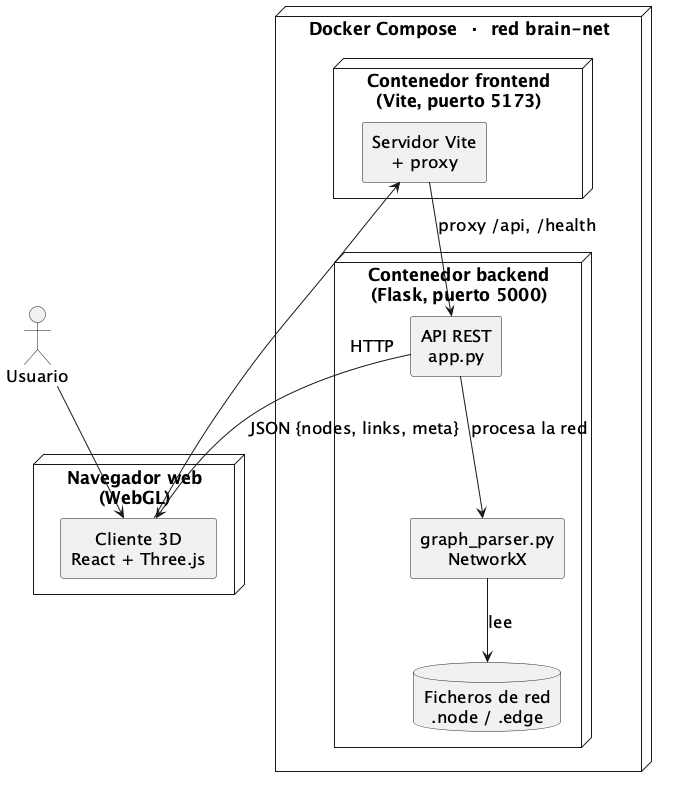
\includegraphics[height=12.5cm]{imagenes/arquitectura}
	\caption{Arquitectura general del sistema.}
	\label{fig:arquitectura}
\end{figure}

En cuanto a los \textbf{patrones de diseño}, la solución se apoya en:

\begin{itemize}
	\item \textbf{Separación de responsabilidades} entre procesamiento de datos (backend) y
		presentación (frontend).
	\item \textbf{Modelo declarativo basado en componentes} en el frontend, propio de React, que
		permite describir la escena 3D y los paneles de la interfaz como componentes reutilizables.
	\item \textbf{Gestión de estado unidireccional} mediante los \textit{hooks} de React, de forma
		que los cambios en los controles (por ejemplo, el umbral de filtrado) se propagan de manera
		predecible a la escena.
\end{itemize}

Durante el análisis se identificaron algunos riesgos técnicos que han condicionado estas
decisiones: la sobrecarga visual por exceso de aristas, la inconsistencia de formatos en los
ficheros de entrada, posibles cuellos de botella en el renderizado y la dependencia del entorno
local. La arquitectura desacoplada y el despliegue con contenedores mitigan principalmente los dos
últimos.

\section{Sprint 1}

El primer \textit{sprint} corresponde a los requisitos de \textbf{Prioridad 1} (RF 1 a RF 4) y
constituye el producto mínimo viable (MVP) de la aplicación. Su objetivo es que un visitante pueda,
sin registro ni instalación de ningún tipo, cargar una red cerebral, procesarla en el \textit{backend}
y visualizarla en 3D, navegando por la escena con la cámara y consultando un panel con las
estadísticas globales de la red.

Al ser el primer \textit{sprint}, además de la funcionalidad propia se ha llevado a cabo toda la
puesta a punto del proyecto: la definición de la arquitectura cliente-servidor, la creación de los
dos servicios (\textit{backend} y \textit{frontend}), la definición del contrato de la API que los
comunica y la configuración del entorno de ejecución con contenedores. Por ello, este \textit{sprint}
sienta las bases técnicas sobre las que se construirán todos los siguientes. En los apartados
siguientes se detalla el diseño de la interfaz, el diseño de los datos, el diseño del software, la
implementación realizada y las pruebas con las que se ha validado.

\subsection{Diseño de la interfaz}

Antes de implementar la interfaz se elaboró un \textbf{boceto (\textit{mockup})} de su distribución,
que sirvió de guía para el desarrollo. La interfaz se ha diseñado como una \textbf{aplicación de una
sola pantalla} en la que la escena 3D ocupa todo el espacio disponible y la información se superpone
en paneles (HUD) situados en las esquinas, de modo que no obstruyan la visualización. Los elementos
principales, mostrados en el \textit{mockup} de la figura~\ref{fig:mockup}, son:

\begin{itemize}
	\item El \textbf{lienzo 3D} central con la red renderizada.
	\item Un \textbf{panel superior izquierdo} con la identidad de la aplicación y las estadísticas
		globales (nodos, conexiones, grupos).
	\item Un \textbf{panel superior derecho} con los controles de visualización.
	\item Una \textbf{leyenda} en la esquina inferior izquierda con la correspondencia entre colores
		y grupos.
\end{itemize}

Se opta por una línea sobria y minimalista: superficies planas, tipografía clara, líneas finas y un
único color de acento, de modo que la atención recaiga sobre la visualización de la red y no sobre
los adornos de la propia interfaz. En este \textit{sprint} no se incluye ninguna pantalla de acceso,
ya que la gestión de usuarios corresponde al Sprint 4.

\begin{figure}[H]
	\centering
	\begin{tikzpicture}[font=\footnotesize]
		% Marco de la pantalla
		\draw[rounded corners=3pt, thick, fill=black!3] (0,0) rectangle (13,8);
		% Etiqueta central de la escena 3D
		\node[align=center, gray] at (6.5,4) {\itshape Lienzo 3D\\\itshape (red renderizada:
		nodos y aristas)};
		% Panel superior izquierdo: identidad + estadísticas
		\draw[rounded corners=2pt, fill=white, draw=black!45] (0.35,5.9) rectangle (4.6,7.65);
		\node[anchor=north west, align=left] at (0.5,7.55)
			{\textbf{Brain Viz}\\[1pt]\footnotesize Estadísticas globales\\\footnotesize Nodos ·
			Conexiones · Grupos};
		% Panel superior derecho: controles
		\draw[rounded corners=2pt, fill=white, draw=black!45] (8.4,5.9) rectangle (12.65,7.65);
		\node[anchor=north west, align=left] at (8.55,7.55)
			{\textbf{Controles}\\[1pt]\footnotesize Mostrar conexiones\\\footnotesize Opacidad ·
			rotación · ejes};
		% Leyenda inferior izquierda
		\draw[rounded corners=2pt, fill=white, draw=black!45] (0.35,0.35) rectangle (4.6,1.8);
		\node[anchor=south west, align=left] at (0.5,0.45)
			{\textbf{Leyenda}\\\footnotesize Grupos / lóbulos (colores)};
	\end{tikzpicture}
	\caption{Boceto (\textit{mockup}) de la distribución de la interfaz principal.}
	\label{fig:mockup}
\end{figure}

\subsection{Diseño de los datos}

Los datos de entrada siguen el formato de \textit{BrainNet Viewer}, descrito en los requisitos de
información [RI 1, RI 2]:

\begin{itemize}
	\item El fichero \texttt{.node} contiene una fila por nodo con las columnas
		\texttt{x  y  z  color\_id  size  label}.
	\item El fichero \texttt{.edge} contiene la matriz de adyacencia $N \times N$ con los pesos de
		las conexiones.
\end{itemize}

La red de ejemplo empleada en este \textit{sprint} es \textbf{AAL90}~\cite{aal}, una parcelación del
cerebro en 90 regiones anatómicas. Su fichero \texttt{.node} contiene, por tanto, 90 filas (una por
región, con sus coordenadas, su lóbulo y su etiqueta) y su fichero \texttt{.edge} una matriz de
adyacencia de $90 \times 90$ con los pesos de conectividad entre cada par de regiones.

\textbf{Almacenamiento en el servidor.} En este primer \textit{sprint} el sistema \textit{no utiliza
base de datos}: las redes públicas precargadas se almacenan directamente como los ficheros
\texttt{.node} y \texttt{.edge} en el servidor. La persistencia mediante base de datos ---necesaria
para las cuentas de usuario y los conjuntos de datos privados, descrita en el requisito de
información [RI 4]--- se introducirá en el Sprint 4, junto con la gestión de usuarios.

\textbf{Modelo interno.} El sistema transforma estas dos fuentes de datos en un modelo interno que no
es un fichero ni una base de datos, sino una \textbf{estructura de datos en memoria}: un grafo (objeto
de la librería de análisis) construido a partir de la matriz de adyacencia, en el que cada nodo se
enriquece con sus coordenadas espaciales, su etiqueta y su grupo. Este grafo es transitorio: existe
únicamente durante el procesamiento de la petición. Como decisión de diseño para reducir la sobrecarga
visual, las aristas cuyo peso es inferior a un umbral mínimo se descartan en esta primera versión, de
modo que solo se representan las conexiones relevantes.

Tras el procesamiento, el \textit{backend} expone la red al \textit{frontend} mediante una estructura
JSON acordada como contrato de la API, con tres bloques:
\begin{itemize}
	\item \texttt{nodes}: lista de nodos, cada uno con su identificador, su etiqueta, sus coordenadas
		$(x, y, z)$ y su grupo o lóbulo.
	\item \texttt{links}: lista de conexiones, cada una con el nodo origen, el nodo destino y el peso
		de la conexión.
	\item \texttt{meta}: metadatos globales de la red, con el número total de nodos y de aristas.
\end{itemize}
Este formato es ligero y directo de consumir por el \textit{frontend}, que lo utiliza tanto para
construir la geometría 3D como para alimentar el panel de estadísticas.

\subsection{Diseño del software}

El backend se organiza en torno a dos módulos principales: un módulo de parseo, responsable de
leer los ficheros, construir el grafo con NetworkX y generar la estructura JSON, y un módulo de
aplicación que define los \textit{endpoints} de la API. La siguiente tabla resume ambos módulos.

\begin{table}[H]
	\centering
	\caption{Módulos del backend en el Sprint 1.}
	\begin{tabularx}{\textwidth}{>{\raggedright\arraybackslash}p{3.2cm} >{\raggedright\arraybackslash}X}
		\toprule
		\textbf{Módulo} & \textbf{Responsabilidad} \\
		\midrule
		\texttt{graph\_parser} & Lee los ficheros \texttt{.node} y \texttt{.edge}, valida su
			consistencia, construye el grafo con NetworkX y genera la estructura JSON de la red. \\
		\addlinespace
		\texttt{app} & Define la aplicación Flask y los \textit{endpoints} de la API
			(\texttt{/health} y \texttt{/api/brain-data}). \\
		\bottomrule
	\end{tabularx}
\end{table}

Los \textit{endpoints} disponibles en este \textit{sprint} son \texttt{/health}, para la
verificación del estado del servicio, y \texttt{/api/brain-data}, que devuelve la red procesada.

En el \textit{frontend}, la aplicación se estructura en componentes siguiendo el modelo declarativo
de React. El componente raíz mantiene el estado global de la interfaz (los metadatos de la red, el
nodo sobre el que se sitúa el cursor y los ajustes de visualización) y contiene la escena 3D y los
paneles del HUD. Un componente de visualización independiente es el encargado de solicitar los datos
a la API y de generar la geometría de nodos y aristas a partir de ellos. La comunicación entre
controles y escena es unidireccional: cuando el usuario modifica un ajuste (por ejemplo, la opacidad
de las aristas), el cambio se propaga desde el estado hacia la escena, que se vuelve a dibujar de
forma reactiva. La figura~\ref{fig:modulos} muestra la modularización del software en este
\textit{sprint}.

\begin{figure}[H]
	\centering
	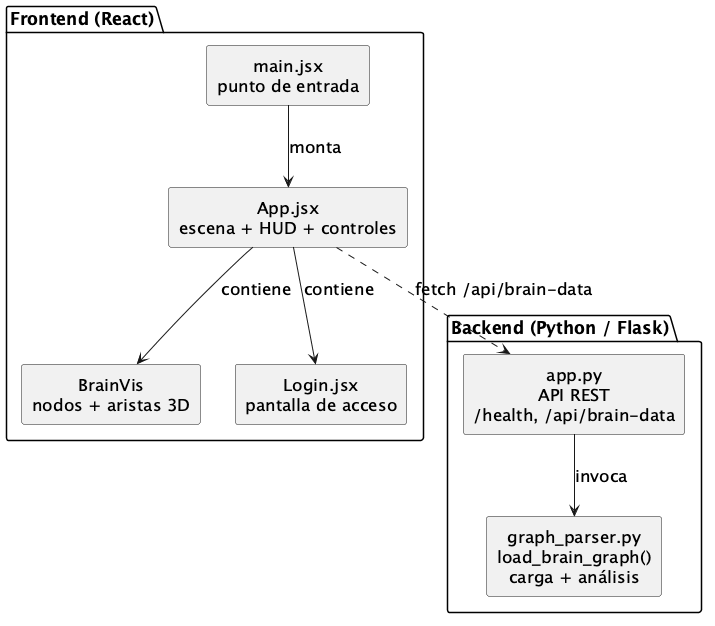
\includegraphics[height=10cm]{imagenes/modulos_sprint1}
	\caption{Modularización del software en el Sprint 1.}
	\label{fig:modulos}
\end{figure}

El modelo de dominio del \textit{backend} se organiza en torno a una clase principal,
\texttt{BrainNetwork}, que representa la red procesada y se compone de sus \texttt{Node}s, sus
\texttt{Edge}s y un bloque de metadatos (\texttt{Meta}). La clase \texttt{GraphParser} es la
responsable de construir esa red a partir de los ficheros de entrada, y la clase \texttt{BrainVizApi}
la expone a través de los \textit{endpoints} de la API. La figura~\ref{fig:clases} recoge este
diagrama de clases (con la nomenclatura en inglés, coherente con la del código).

\begin{figure}[H]
	\centering
	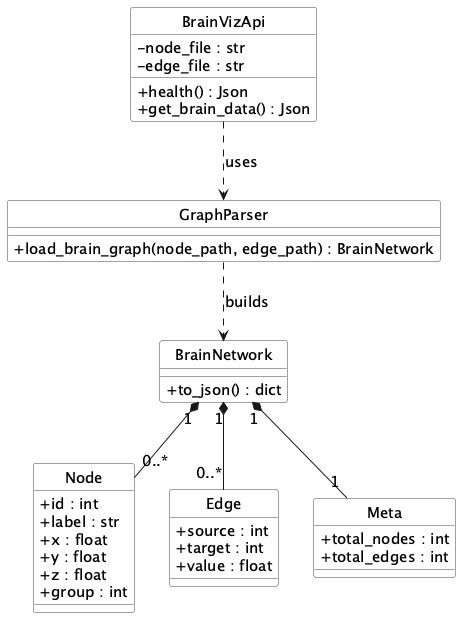
\includegraphics[height=9.5cm]{imagenes/clases_sprint1}
	\caption{Diagrama de clases del modelo de dominio del backend (Sprint 1).}
	\label{fig:clases}
\end{figure}

El flujo de la carga inicial de la red es el siguiente: al abrir la aplicación, el frontend realiza
una petición a \texttt{/api/brain-data}; el backend lee los ficheros de la red, construye el grafo,
lo serializa a JSON y lo devuelve; el frontend recibe los datos, calcula la geometría y renderiza la
escena, actualizando además el panel de estadísticas. Este flujo se representa en el diagrama de
secuencia de la figura~\ref{fig:secuencia}.

\begin{figure}[H]
	\centering
	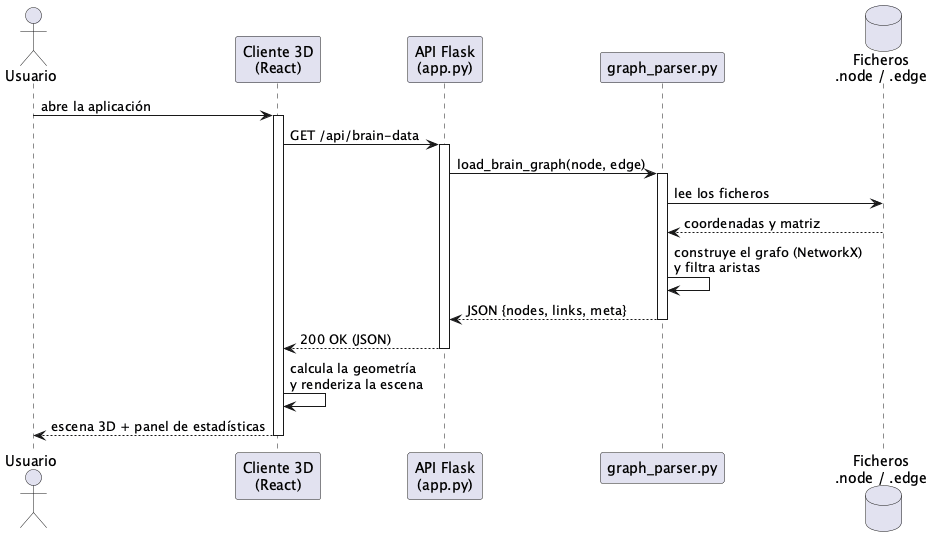
\includegraphics[width=\textwidth]{imagenes/sec_carga_red}
	\caption{Diagrama de secuencia de la carga y visualización de una red.}
	\label{fig:secuencia}
\end{figure}

Conviene señalar una limitación de este diseño inicial: tal y como está planteado, cada petición de
una red reconstruye el grafo y su JSON desde los ficheros, de modo que visualizar la misma red muchas
veces repite el mismo trabajo. Para las redes públicas, que no cambian, esto es ineficiente. Una
mejora prevista ---que se abordará al introducir la persistencia en el Sprint 4--- es \textbf{construir
la red y su JSON una sola vez y almacenar el resultado} (en una caché o en la base de datos) para
reutilizarlo en las siguientes peticiones, evitando así el reprocesamiento.

\subsection{Implementación}

La implementación de este \textit{sprint} cubre los requisitos de Prioridad 1 (RF 1 a RF 4) y se
reparte entre los dos servicios de la aplicación, el \textit{backend} y el \textit{frontend}, más la
configuración del entorno de despliegue. A continuación se detalla el trabajo realizado en cada uno.

\subsubsection*{Backend: procesamiento y API (RF 1, RF 2.1)}

El \textit{backend} se ha implementado en Python con Flask y se organiza en los dos módulos descritos
anteriormente. El módulo de parseo es el núcleo del procesamiento y realiza la siguiente secuencia de
tareas:

\begin{enumerate}
	\item \textbf{Validación de entrada.} Comprueba que existen los ficheros de nodos y de aristas y,
		en caso contrario, informa del error sin que el servicio se detenga.
	\item \textbf{Lectura de los datos.} Lee el fichero de nodos como una tabla, admitiendo tanto
		espacios como tabuladores como separadores, y carga la matriz de adyacencia.
	\item \textbf{Construcción del grafo.} Convierte la matriz de adyacencia en un grafo no dirigido
		mediante NetworkX y asocia a cada nodo sus atributos (coordenadas, etiqueta y grupo).
	\item \textbf{Filtrado de aristas.} Descarta las conexiones con un peso por debajo del umbral
		mínimo, para no saturar la visualización con enlaces poco significativos.
	\item \textbf{Serialización.} Genera la estructura JSON con los bloques \texttt{nodes},
		\texttt{links} y \texttt{meta} que consume el \textit{frontend}.
\end{enumerate}

El núcleo de este procesamiento es breve gracias a NetworkX. El siguiente fragmento resume la
construcción del grafo a partir de la matriz de adyacencia y el filtrado de aristas por umbral:

\begin{lstlisting}[language=Python, basicstyle=\footnotesize\ttfamily, keywordstyle=\color{blue!60!black}, commentstyle=\color{gray}, showstringspaces=false, frame=single, columns=fullflexible]
# Grafo no dirigido a partir de la matriz de adyacencia
G = nx.from_numpy_array(adj_matrix, create_using=nx.Graph)

# Filtrado de aristas por umbral y serializacion a JSON
links = [
    {"source": u, "target": v, "value": w}
    for u, v, w in G.edges.data("weight")
    if w > THRESHOLD
]
\end{lstlisting}

El uso de NetworkX en esta fase, aunque en el Sprint 1 se limita a la construcción del grafo, deja
preparada la infraestructura para el cálculo de métricas de teoría de grafos en los \textit{sprints}
posteriores. Sobre este módulo, la aplicación Flask define los dos \textit{endpoints} de la API.
Además de responder en JSON, ambos incorporan una negociación de contenido que permite devolver una
página HTML legible cuando se accede a ellos desde el navegador, lo que facilita la depuración durante
el desarrollo. La comunicación con el \textit{frontend} se habilita mediante CORS.

\subsubsection*{Frontend: visualización e interacción (RF 2, RF 3, RF 4)}

El \textit{frontend} se ha implementado en React con Vite como herramienta de construcción, y utiliza
Three.js a través de \textit{react-three-fiber} y su librería de utilidades \textit{drei} para el
renderizado 3D declarativo. Al iniciarse, la aplicación solicita la red al \textit{endpoint}
\texttt{/api/brain-data} y, con los datos recibidos, construye la escena:

\begin{itemize}
	\item \textbf{Nodos (RF 2).} Cada nodo se representa como una esfera situada en sus coordenadas
		anatómicas, coloreada según su grupo o lóbulo mediante una paleta categórica, de forma que las
		regiones de una misma agrupación comparten color.
	\item \textbf{Aristas (RF 2).} Las conexiones se dibujan como segmentos de línea entre los nodos
		que unen. Su opacidad es ajustable, lo que permite atenuarlas para percibir mejor la estructura
		en redes densas.
	\item \textbf{Navegación (RF 3).} La cámara se controla con los controles de órbita de Three.js,
		que permiten rotar, hacer zoom y desplazar la escena, con amortiguación para un movimiento
		suave y límites de acercamiento y alejamiento para no perder el modelo de vista.
	\item \textbf{Panel de estadísticas (RF 4).} Un panel superpuesto (HUD) muestra en tiempo real el
		número de nodos, de conexiones y de grupos de la red activa.
\end{itemize}

La interfaz se completa con un panel de controles de visualización (mostrar u ocultar las conexiones,
activar la rotación automática de la escena, mostrar los ejes de referencia y ajustar la opacidad de
las aristas mediante un deslizador), una leyenda que asocia cada color a su grupo, la información
emergente al situar el cursor sobre un nodo y unos estados de carga y de error que informan al usuario
mientras se obtienen los datos o si estos no están disponibles. Todo ello sigue una línea visual sobria
y minimalista, coherente con la naturaleza científica de la herramienta.

\subsection{Despliegue y control de versiones}

Ambos servicios se han contenerizado y se orquestan con Docker Compose, que los levanta en una red
interna común. El navegador solo se comunica con el \textit{frontend}, y las peticiones a la API se
redirigen internamente al \textit{backend} mediante un \textit{proxy}, evitando así problemas de
CORS y de configuración de puertos en el cliente. El entorno está preparado para el desarrollo con
recarga en caliente, de modo que los cambios en el código se reflejan de inmediato sin reconstruir las
imágenes. El detalle del procedimiento de instalación y ejecución se recoge en el manual de
instalación.

El desarrollo se ha gestionado con control de versiones mediante Git, alojando el repositorio en
GitHub y registrando el avance con \textit{commits} sucesivos a lo largo del \textit{sprint}. El
código completo puede consultarse en el repositorio público del proyecto:
\url{https://github.com/pablomlz/brain-viz}.

\subsection{Pruebas}

La estrategia de pruebas de cada \textit{sprint} combina tres tipos de pruebas: pruebas de caja
blanca (unitarias) sobre el código, pruebas de caja negra (de integración) sobre la comunicación
entre servicios y pruebas de validación (o de aceptación) que comprueban el cumplimiento de los
requisitos. Conviene recordar que, en ingeniería del software, una prueba se considera exitosa
cuando es capaz de \emph{descubrir un error}; por ello, al final de este apartado se describen
algunos de los errores detectados y cómo se corrigieron.

\subsubsection*{Pruebas de caja blanca (unitarias)}

Se han probado de forma aislada las funciones del módulo de parseo, comprobando que, ante ficheros
correctos, el grafo resultante tiene el número esperado de nodos y aristas y que los atributos de los
nodos (coordenadas, etiqueta y grupo) se corresponden con los del fichero de entrada. También se han
probado los casos límite: ficheros inexistentes, matriz de adyacencia con dimensiones que no
coinciden con el número de nodos y valores fuera de rango.

\subsubsection*{Pruebas de caja negra (de integración)}

Se ha verificado la comunicación entre el \textit{frontend} y el \textit{backend} a través de la API,
sin conocer la implementación interna: se comprueba que el \textit{endpoint} \texttt{/api/brain-data}
responde con un JSON cuya estructura respeta el contrato acordado (\texttt{nodes}, \texttt{links} y
\texttt{meta}) y que el \textit{frontend} es capaz de renderizar la escena a partir de esa respuesta.

\subsubsection*{Pruebas de validación (de aceptación)}

Por último, se han diseñado pruebas de validación alineadas con los criterios del capítulo de
requisitos, que verifican que cada requisito de Prioridad~1 se comporta como se espera. La
tabla~\ref{tab:pruebas} recoge estas pruebas, el requisito que validan y su resultado.

\begin{table}[H]
	\centering
	\caption{Pruebas de validación del Sprint 1.}
	\label{tab:pruebas}
	\small
	\begin{tabularx}{\textwidth}{>{\raggedright\arraybackslash}p{1.4cm} >{\raggedright\arraybackslash}X >{\raggedright\arraybackslash}X >{\centering\arraybackslash}p{1.6cm}}
		\toprule
		\textbf{Prueba} & \textbf{Descripción} & \textbf{Resultado esperado} & \textbf{Estado} \\
		\midrule
		P-01 (RF 2.1) & Petición a \texttt{/health} y a \texttt{/api/brain-data}. &
			\texttt{/health} responde \texttt{ok}; \texttt{/api/brain-data} devuelve un JSON válido
			con \texttt{nodes}, \texttt{links} y \texttt{meta}. & Correcto \\
		\addlinespace
		P-02 (RF 1, RF 2) & Carga y renderizado del atlas AAL90. &
			Los 90 nodos se sitúan en sus coordenadas y las aristas conectan los nodos correctos. &
			Correcto \\
		\addlinespace
		P-03 (RF 2.1) & Carga con ficheros de dimensiones incongruentes. &
			El sistema detecta el error y no cae (respuesta de error controlada). & Correcto \\
		\addlinespace
		P-04 (RF 3) & Navegación con la cámara (rotar, zoom y paneo). &
			La cámara responde de forma fluida, con amortiguación y límites de zoom. & Correcto \\
		\addlinespace
		P-05 (RF 4) & Comprobación del panel de estadísticas. &
			El HUD muestra el número de nodos, aristas y grupos coherente con los datos de entrada. &
			Correcto \\
		\bottomrule
	\end{tabularx}
\end{table}

\subsubsection*{Errores detectados y corregidos}

Durante las pruebas se detectaron y corrigieron varios errores, lo que confirma su utilidad. Los más
relevantes fueron:

\begin{itemize}
	\item \textbf{Etiqueta incorrecta en la información del nodo.} Al situar el cursor sobre un nodo, la
		información emergente mostraba un texto genérico (``Nodo \#\textit{i}'') en lugar del nombre de
		la región. La prueba de la interacción reveló que el código leía un campo inexistente
		(\texttt{name}) en vez del campo real del contrato de la API (\texttt{label}); se corrigió
		haciendo que leyera \texttt{label}.
	\item \textbf{Caída ante ficheros incongruentes.} Una primera versión no comprobaba que las
		dimensiones de la matriz de adyacencia coincidieran con el número de nodos, lo que provocaba un
		error no controlado. La prueba de caja blanca con ficheros incongruentes lo puso de manifiesto
		y se añadió la validación correspondiente, que ahora devuelve un error controlado [RNF 3].
\end{itemize}

Estas pruebas se han realizado de forma manual sobre el entorno desplegado con contenedores. En los
sucesivos \textit{sprints} se completarán con pruebas automatizadas del \textit{backend} y con la
medición del rendimiento gráfico (FPS) para verificar el requisito no funcional de fluidez [RNF 1].

\subsubsection*{Validación por parte del cliente}

Al finalizar el \textit{sprint} se realiza la prueba fundamental de todo desarrollo ágil: la
validación por parte del cliente, cuyo papel asume el director del proyecto. Para que pueda probar la
aplicación de forma cómoda ---y, más adelante, también el tribunal---, el Sprint~1 se despliega en un
servidor público accesible y se le facilita su URL.
% NOTA: insertar aquí la URL del despliegue una vez publicado el Sprint 1 en el servidor.

\section{Sprint 2}

El segundo \textit{sprint} corresponde a los requisitos de \textbf{Prioridad 2} (RF 5, RF 6 y RF 7) y
constituye el núcleo de la exploración interactiva de la red. Mientras que el Sprint~1 permitía
\emph{ver} la red, este \textit{sprint} permite \emph{explorarla}: reducir su complejidad visual
filtrando las conexiones menos relevantes (RF 5), consultar la información concreta de una región
seleccionándola con el ratón (RF 6) y distinguir las agrupaciones anatómicas mediante el coloreado y
su leyenda (RF 7).

De los tres requisitos, el RF 7 ya quedó cubierto durante el Sprint~1, puesto que el coloreado por
grupo y su leyenda eran necesarios para que la visualización inicial resultara legible; en este
\textit{sprint} se da por consolidado y el esfuerzo se concentra en los otros dos. El desarrollo ha
requerido modificar tanto el \textit{backend} ---que hasta ahora aplicaba un umbral fijo y no
proporcionaba toda la información de cada nodo--- como el \textit{frontend}, donde reside la
interacción.

\subsection{Diseño de la interfaz}

El diseño parte del establecido en el Sprint~1 y añade dos elementos, manteniendo el principio de que
la escena 3D ocupe todo el espacio y la información se superponga en paneles que no la obstruyan:

\begin{itemize}
	\item Un \textbf{control deslizante de umbral} en el panel de controles (RF 5). Se sitúa en primer
		lugar por ser el control con mayor impacto sobre la visualización, y muestra junto a él el valor
		numérico del umbral activo.
	\item Un \textbf{panel de información del nodo seleccionado} (RF 6), que aparece bajo el panel de
		controles únicamente cuando hay un nodo seleccionado y puede cerrarse explícitamente. Se ha
		optado por un panel lateral persistente, en lugar de una ventana emergente, para que el usuario
		pueda seguir rotando la escena mientras consulta los datos de la región.
\end{itemize}

Además, el contador de conexiones del panel de estadísticas pasa a mostrar la relación
\textit{visibles / totales}, de modo que el usuario perciba en todo momento qué proporción de la red
está viendo. La figura~\ref{fig:mockup-s2} recoge el boceto de la interfaz resultante, con los dos
elementos nuevos destacados.

\begin{figure}[H]
	\centering
	\begin{tikzpicture}[font=\footnotesize]
		% Marco de la pantalla
		\draw[rounded corners=3pt, thick, fill=black!3] (0,0) rectangle (13,8.6);
		% Escena 3D
		\node[align=center, gray] at (4.3,4.2) {\itshape Lienzo 3D\\\itshape (nodo seleccionado
		\itshape resaltado)};
		% Panel superior izquierdo: estadísticas
		\draw[rounded corners=2pt, fill=white, draw=black!45] (0.35,6.5) rectangle (4.6,8.25);
		\node[anchor=north west, align=left] at (0.5,8.15)
			{\textbf{Brain Viz}\\[1pt]\footnotesize Nodos · Grupos\\\footnotesize
			\textbf{Conexiones: visibles / totales}};
		% Panel superior derecho: controles (con umbral destacado)
		\draw[rounded corners=2pt, fill=white, draw=black!45] (8.4,6.1) rectangle (12.65,8.25);
		\node[anchor=north west, align=left] at (8.55,8.15)
			{\textbf{Controles}\\[2pt]\footnotesize\textbf{Umbral de peso} \; \tikz[baseline=-0.5ex]{
				\draw[black!45] (0,0) -- (1.5,0); \fill[black!70] (0.95,0) circle (2.2pt);}\\
			\footnotesize Conexiones · rotación · ejes\\\footnotesize Opacidad};
		% Panel derecho: nodo seleccionado (nuevo)
		\draw[rounded corners=2pt, fill=white, draw=black!45, very thick] (8.4,2.6) rectangle (12.65,5.7);
		\node[anchor=north west, align=left] at (8.55,5.6)
			{\textbf{Nodo seleccionado} \hfill $\times$\\[2pt]\footnotesize Etiqueta de la región\\
			\footnotesize Identificador · Grupo\\\footnotesize \textbf{Grado}\\
			\footnotesize Coordenadas X, Y, Z};
		% Leyenda inferior izquierda
		\draw[rounded corners=2pt, fill=white, draw=black!45] (0.35,0.35) rectangle (4.6,1.8);
		\node[anchor=south west, align=left] at (0.5,0.45)
			{\textbf{Leyenda}\\\footnotesize Grupos / lóbulos (colores)};
	\end{tikzpicture}
	\caption{Boceto de la interfaz del Sprint 2. En trazo grueso, el nuevo panel de información del
	nodo seleccionado; en el panel de controles se incorpora el umbral de peso.}
	\label{fig:mockup-s2}
\end{figure}

\subsection{Diseño de los datos}

Las dos funcionalidades de este \textit{sprint} obligan a revisar el contrato de la API definido en
el Sprint~1, ya que la información que enviaba el servidor resultaba insuficiente:

\begin{itemize}
	\item \textbf{La red debe enviarse completa.} En el Sprint~1 el servidor descartaba las aristas
		por debajo de un umbral fijo. Si el umbral pasa a ser del usuario, el servidor no puede decidir
		de antemano qué aristas sobran: debe enviar todas las conexiones existentes y dejar el filtrado
		al cliente. En la red de ejemplo esto supone pasar de 365 a 411 aristas.
	\item \textbf{Cada nodo incorpora su grado} (\texttt{degree}), es decir, su número de conexiones en
		la red completa. Es un dato que el panel de información debe mostrar (RF 6) y que se calcula en
		el servidor con la librería de análisis de grafos, evitando que el cliente tenga que recorrer
		toda la lista de aristas.
	\item \textbf{Los metadatos incorporan el rango de pesos} (\texttt{min\_weight} y
		\texttt{max\_weight}). Con ellos, el control de umbral se calibra con los pesos reales de la red
		en lugar de asumir un rango fijo, de modo que la interfaz funcione igual con una red cuyos pesos
		sean correlaciones en $[0,1]$ que con otra cuyos valores sean, por ejemplo, recuentos de fibras
		de orden muy distinto. La interfaz muestra además los extremos del rango junto al control, para
		que el usuario sepa entre qué valores se mueve la red que está explorando.
	\item \textbf{Las aristas se envían ordenadas por peso descendente.} Esta decisión, que no altera
		la información transmitida, es la que permite implementar el filtrado de forma eficiente, como
		se explica en el diseño del software.
\end{itemize}

Un matiz importante del modelo de datos es que ahora se distingue entre \emph{existir} y \emph{ser
visible}: una arista existe si su peso es mayor que cero en la matriz de adyacencia ---y como tal
cuenta para el grado de los nodos---, mientras que su visibilidad depende del umbral que fije el
usuario en cada momento. Por ello, el grado que muestra el panel de información se refiere siempre a
la red completa y no varía al mover el control de umbral. La figura~\ref{fig:clases-s2} recoge el
modelo de datos resultante, con los atributos añadidos en este \textit{sprint} destacados.

\begin{figure}[H]
	\centering
	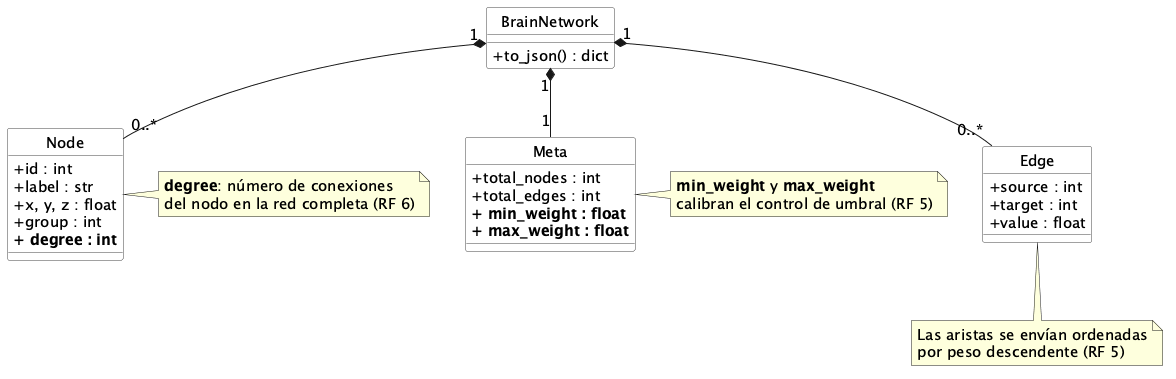
\includegraphics[width=\textwidth]{imagenes/clases_sprint2}
	\caption{Modelo de datos tras el Sprint 2, con los atributos añadidos para el filtrado (RF 5) y la
	inspección de nodos (RF 6).}
	\label{fig:clases-s2}
\end{figure}

\subsection{Diseño del software}

La característica que define este \textit{sprint} desde el punto de vista del diseño es que
\textbf{ninguna de las dos interacciones requiere comunicarse con el servidor}. Tanto el filtrado
como la selección operan sobre los datos que el cliente ya ha recibido, lo que resulta imprescindible
para cumplir el requisito de que el filtrado se aplique \emph{en tiempo real} (RF 5): una petición
por cada movimiento del control deslizante haría la interacción inviable.

El punto delicado es cómo aplicar el umbral sin penalizar el rendimiento. La solución directa
---recorrer las aristas y reconstruir la geometría cada vez que el usuario mueve el control--- obliga
a recalcular y volver a enviar a la tarjeta gráfica miles de vértices en cada fotograma. En su lugar
se ha adoptado la siguiente estrategia, apoyada en que el servidor entrega las aristas ordenadas por
peso descendente:

\begin{enumerate}
	\item La geometría de las aristas se construye \textbf{una sola vez} al cargar la red, con todas
		las conexiones y en orden de peso decreciente.
	\item Al fijar un umbral, las aristas que lo superan son necesariamente las \textbf{primeras} de
		esa secuencia ordenada. Determinar cuántas son se reduce entonces a localizar la posición de la
		primera arista que no alcanza el umbral, lo que se resuelve con una \textbf{búsqueda binaria},
		de coste $O(\log E)$ sobre el número de aristas $E$, en lugar de recorrer la lista completa.
	\item Basta entonces con indicar al motor gráfico cuántos elementos debe dibujar
		(\textit{rango de dibujado}), operación de \textbf{coste constante} que no modifica la
		geometría ni vuelve a enviarla a la tarjeta gráfica.
\end{enumerate}

De este modo, mover el control deslizante no implica reconstruir nada: su coste es logarítmico en el
número de aristas y prácticamente independiente del tamaño de la red, por lo que la escena responde
de forma inmediata. La figura~\ref{fig:sec-s2} muestra el diagrama de secuencia de ambas
interacciones.

\begin{figure}[H]
	\centering
	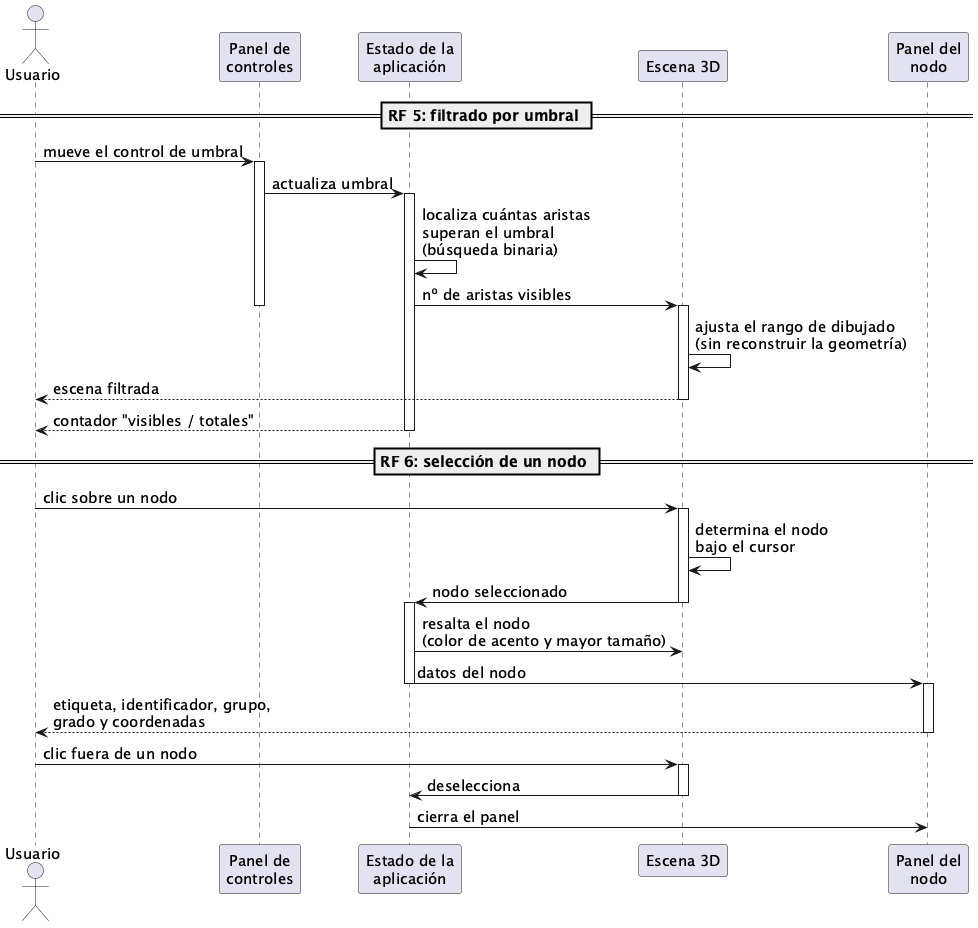
\includegraphics[width=\textwidth]{imagenes/sec_interaccion_sprint2}
	\caption{Diagrama de secuencia del filtrado por umbral (RF 5) y de la selección de un nodo (RF 6).}
	\label{fig:sec-s2}
\end{figure}

En cuanto a la selección (RF 6), se aprovecha la detección de intersecciones (\textit{raycasting})
que ofrece la librería de renderizado: al hacer clic, se determina qué nodo se encuentra bajo el
cursor y su identificador se guarda en el estado de la aplicación. A partir de ahí, y gracias al
modelo declarativo, tanto el resaltado del nodo en la escena como la aparición del panel de
información son consecuencia automática de ese cambio de estado. La deselección se resuelve
capturando los clics que no impactan sobre ningún nodo.

\subsection{Implementación}

\subsubsection*{Backend: red completa, grado y rango de pesos (RF 5, RF 6)}

En el módulo de parseo se ha eliminado el umbral fijo y se ha añadido el cálculo del grado. Como las
aristas de peso nulo no representan conexiones reales, se eliminan del grafo antes de calcular los
grados, de modo que el grado obtenido sea el correcto:

\begin{lstlisting}[language=Python, basicstyle=\footnotesize\ttfamily, keywordstyle=\color{blue!60!black}, commentstyle=\color{gray}, showstringspaces=false, frame=single, columns=fullflexible]
# Las aristas de peso nulo no representan conexion: se eliminan del grafo
# para que el grado de cada nodo sea el real
sin_conexion = [(u, v) for u, v, w in G.edges(data='weight') if w <= MIN_WEIGHT]
G.remove_edges_from(sin_conexion)

# Grado de cada nodo en la red completa (RF 6)
"degree": int(G.degree(i)),

# Aristas ordenadas por peso descendente: permite el filtrado eficiente (RF 5)
links_data.sort(key=lambda link: link["value"], reverse=True)
\end{lstlisting}

Se ha reforzado además la validación de los ficheros de entrada, comprobando que la matriz de
adyacencia sea cuadrada y que su dimensión coincida con el número de nodos declarados, y devolviendo
un error descriptivo en caso contrario [RNF 3].

\subsubsection*{Frontend: filtrado en tiempo real (RF 5)}

El componente de visualización construye la geometría una única vez y aplica el umbral ajustando el
rango de dibujado, siguiendo la estrategia descrita en el diseño:

\begin{lstlisting}[language=JavaScript, basicstyle=\footnotesize\ttfamily, keywordstyle=\color{blue!60!black}, commentstyle=\color{gray}, showstringspaces=false, frame=single, columns=fullflexible]
// Las aristas llegan ordenadas por peso: las visibles son siempre las
// primeras, asi que basta con ajustar el rango de dibujado (2 vertices/arista)
useEffect(() => {
  if (linesGeometry) linesGeometry.setDrawRange(0, settings.visibleLinks * 2);
}, [linesGeometry, settings.visibleLinks]);
\end{lstlisting}

El número de aristas visibles se obtiene con la búsqueda binaria descrita en el diseño, y alimenta
tanto la escena como el contador \textit{visibles / totales} del panel de estadísticas:

\begin{lstlisting}[language=JavaScript, basicstyle=\footnotesize\ttfamily, keywordstyle=\color{blue!60!black}, commentstyle=\color{gray}, showstringspaces=false, frame=single, columns=fullflexible]
// Posicion de la primera arista que ya no alcanza el umbral: O(log E)
function contarVisibles(links, umbral) {
  let ini = 0, fin = links.length;
  while (ini < fin) {
    const medio = (ini + fin) >> 1;
    if (links[medio].value >= umbral) ini = medio + 1;
    else fin = medio;
  }
  return ini;
}
\end{lstlisting}

\subsubsection*{Frontend: selección e inspección de nodos (RF 6)}

Cada nodo responde al evento de clic registrando su índice en el estado; volver a pulsar sobre el
mismo nodo lo deselecciona, y un clic fuera de cualquier nodo cierra la selección. El nodo
seleccionado se resalta con el color de acento de la interfaz y un tamaño mayor, mientras que el panel
muestra su etiqueta anatómica, identificador, grupo, grado y coordenadas.

Las figuras~\ref{fig:s2-umbral} y~\ref{fig:s2-seleccion} muestran el resultado de la implementación
sobre la red de ejemplo: la primera compara la red completa con la red filtrada, y la segunda recoge
la selección de una región con su panel de información.

\begin{figure}[H]
	\centering
	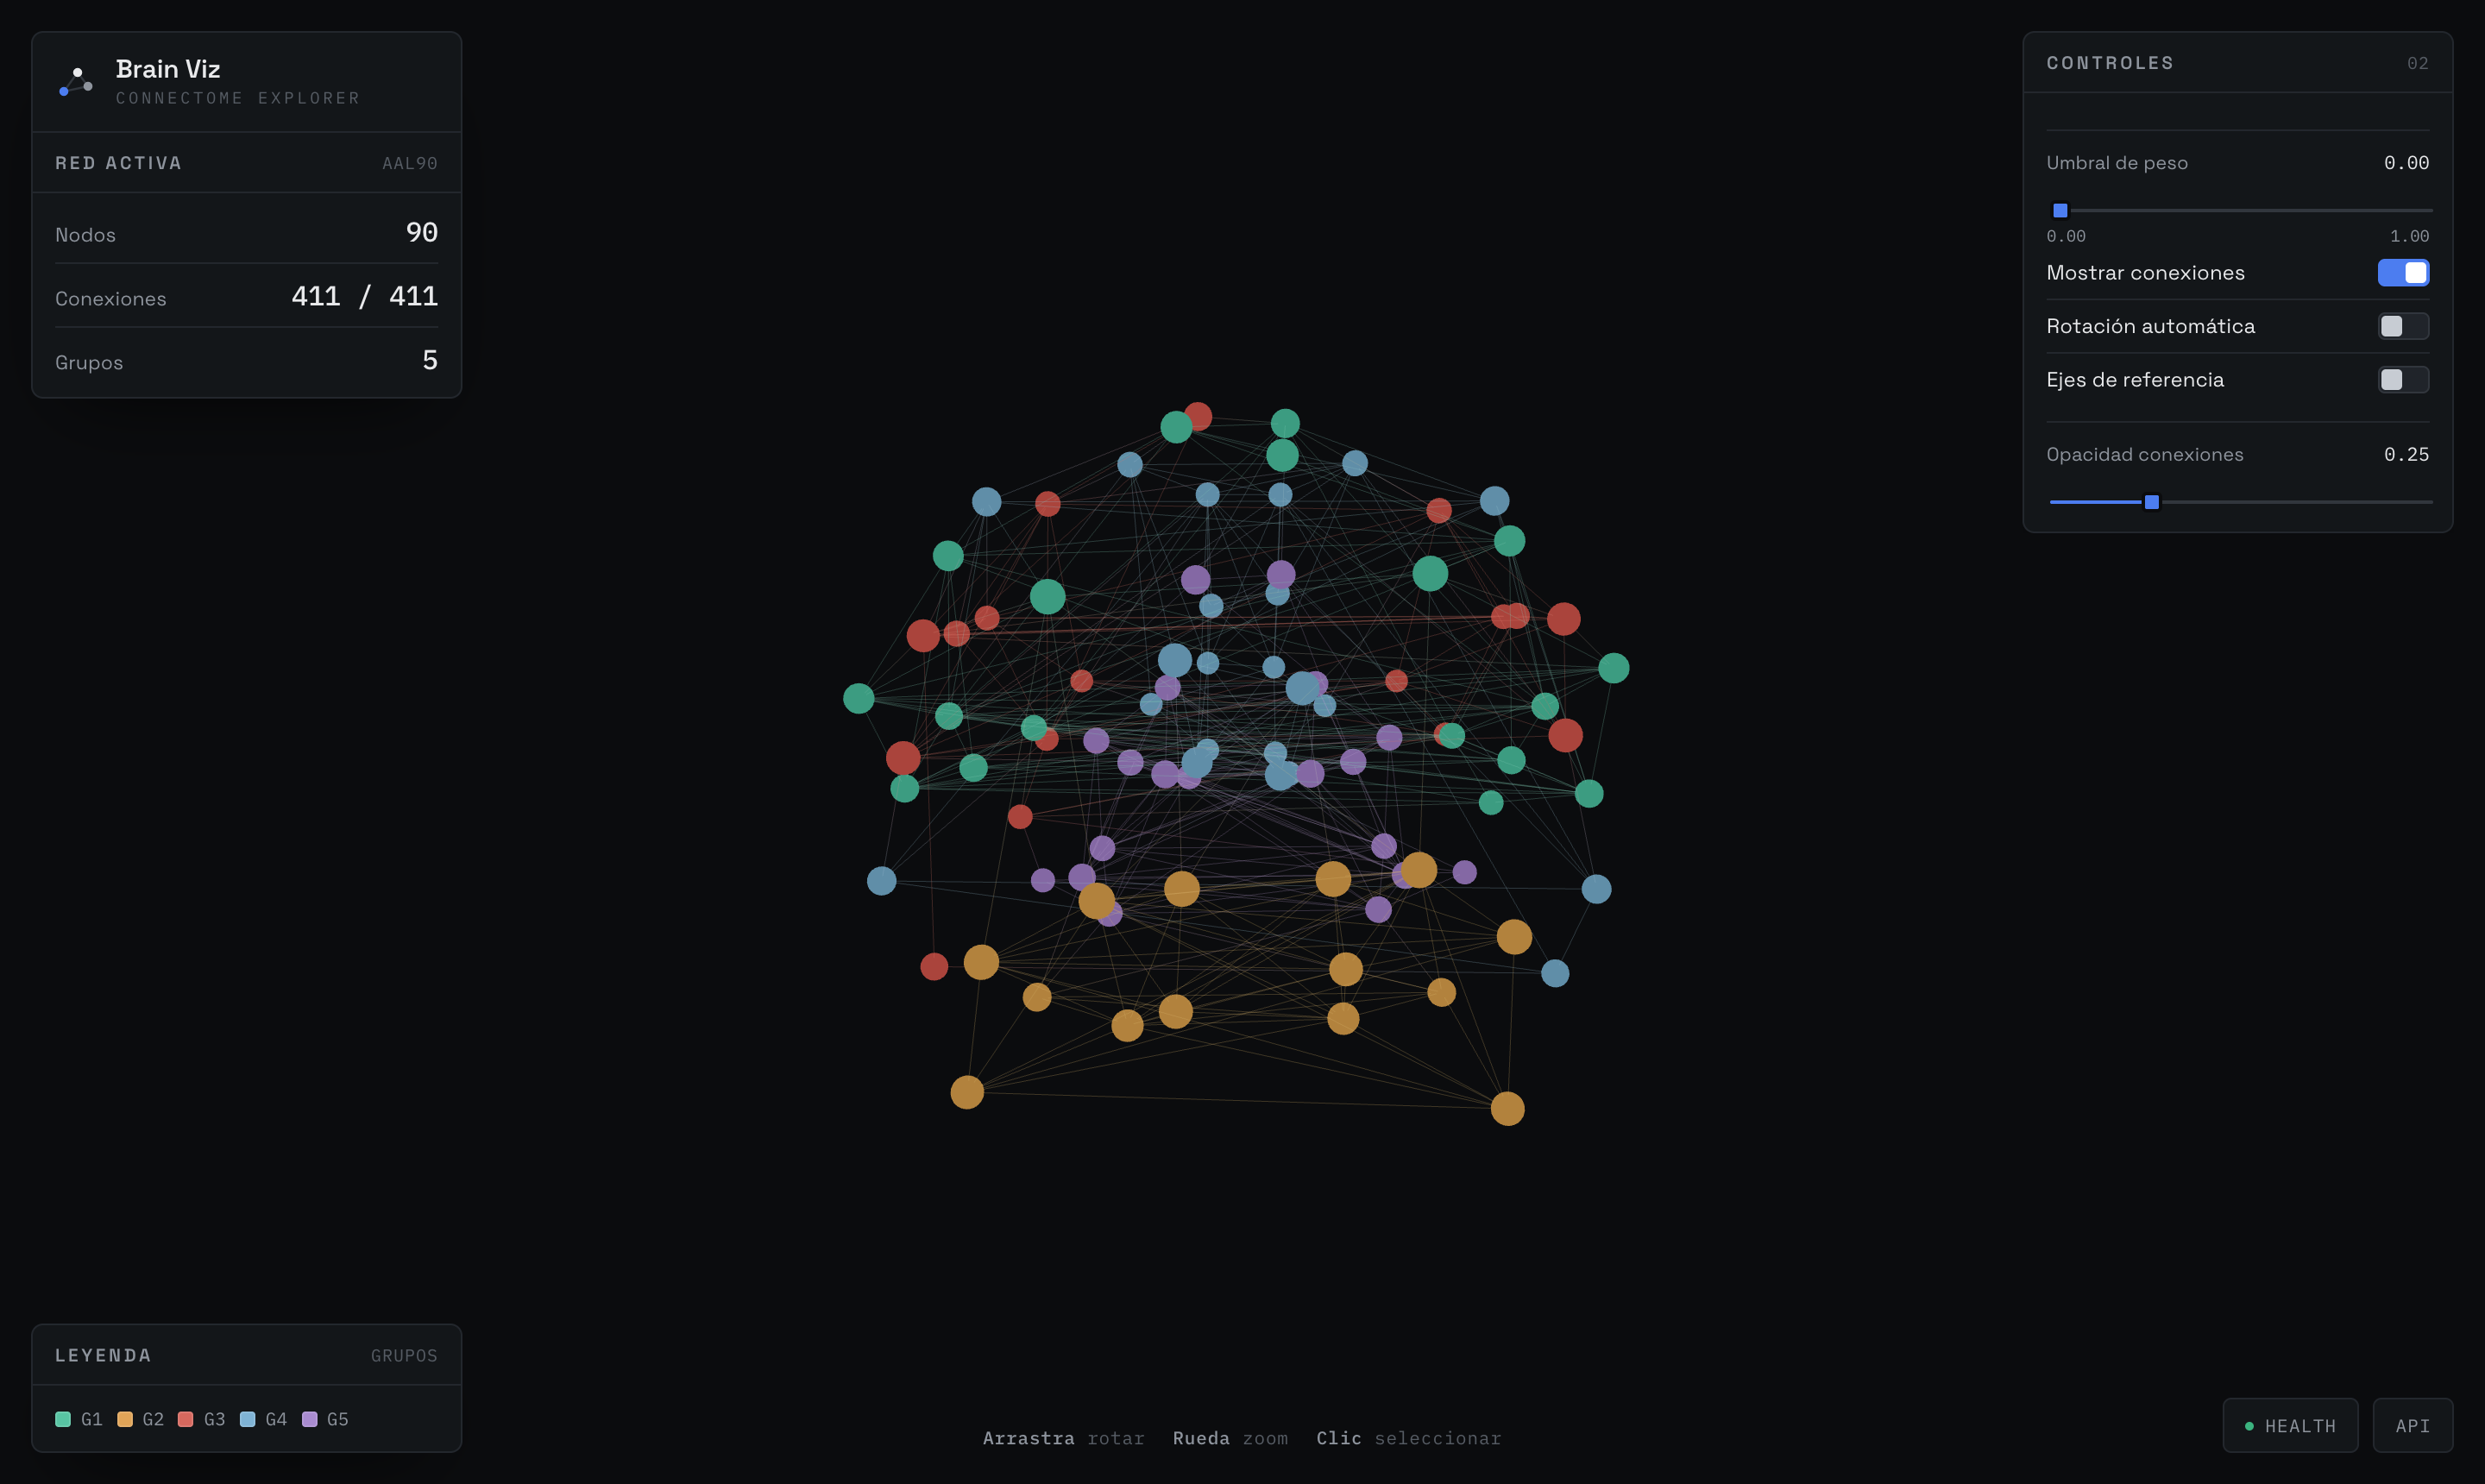
\includegraphics[width=0.86\textwidth]{imagenes/app_s2_umbral_bajo}\\[6pt]
	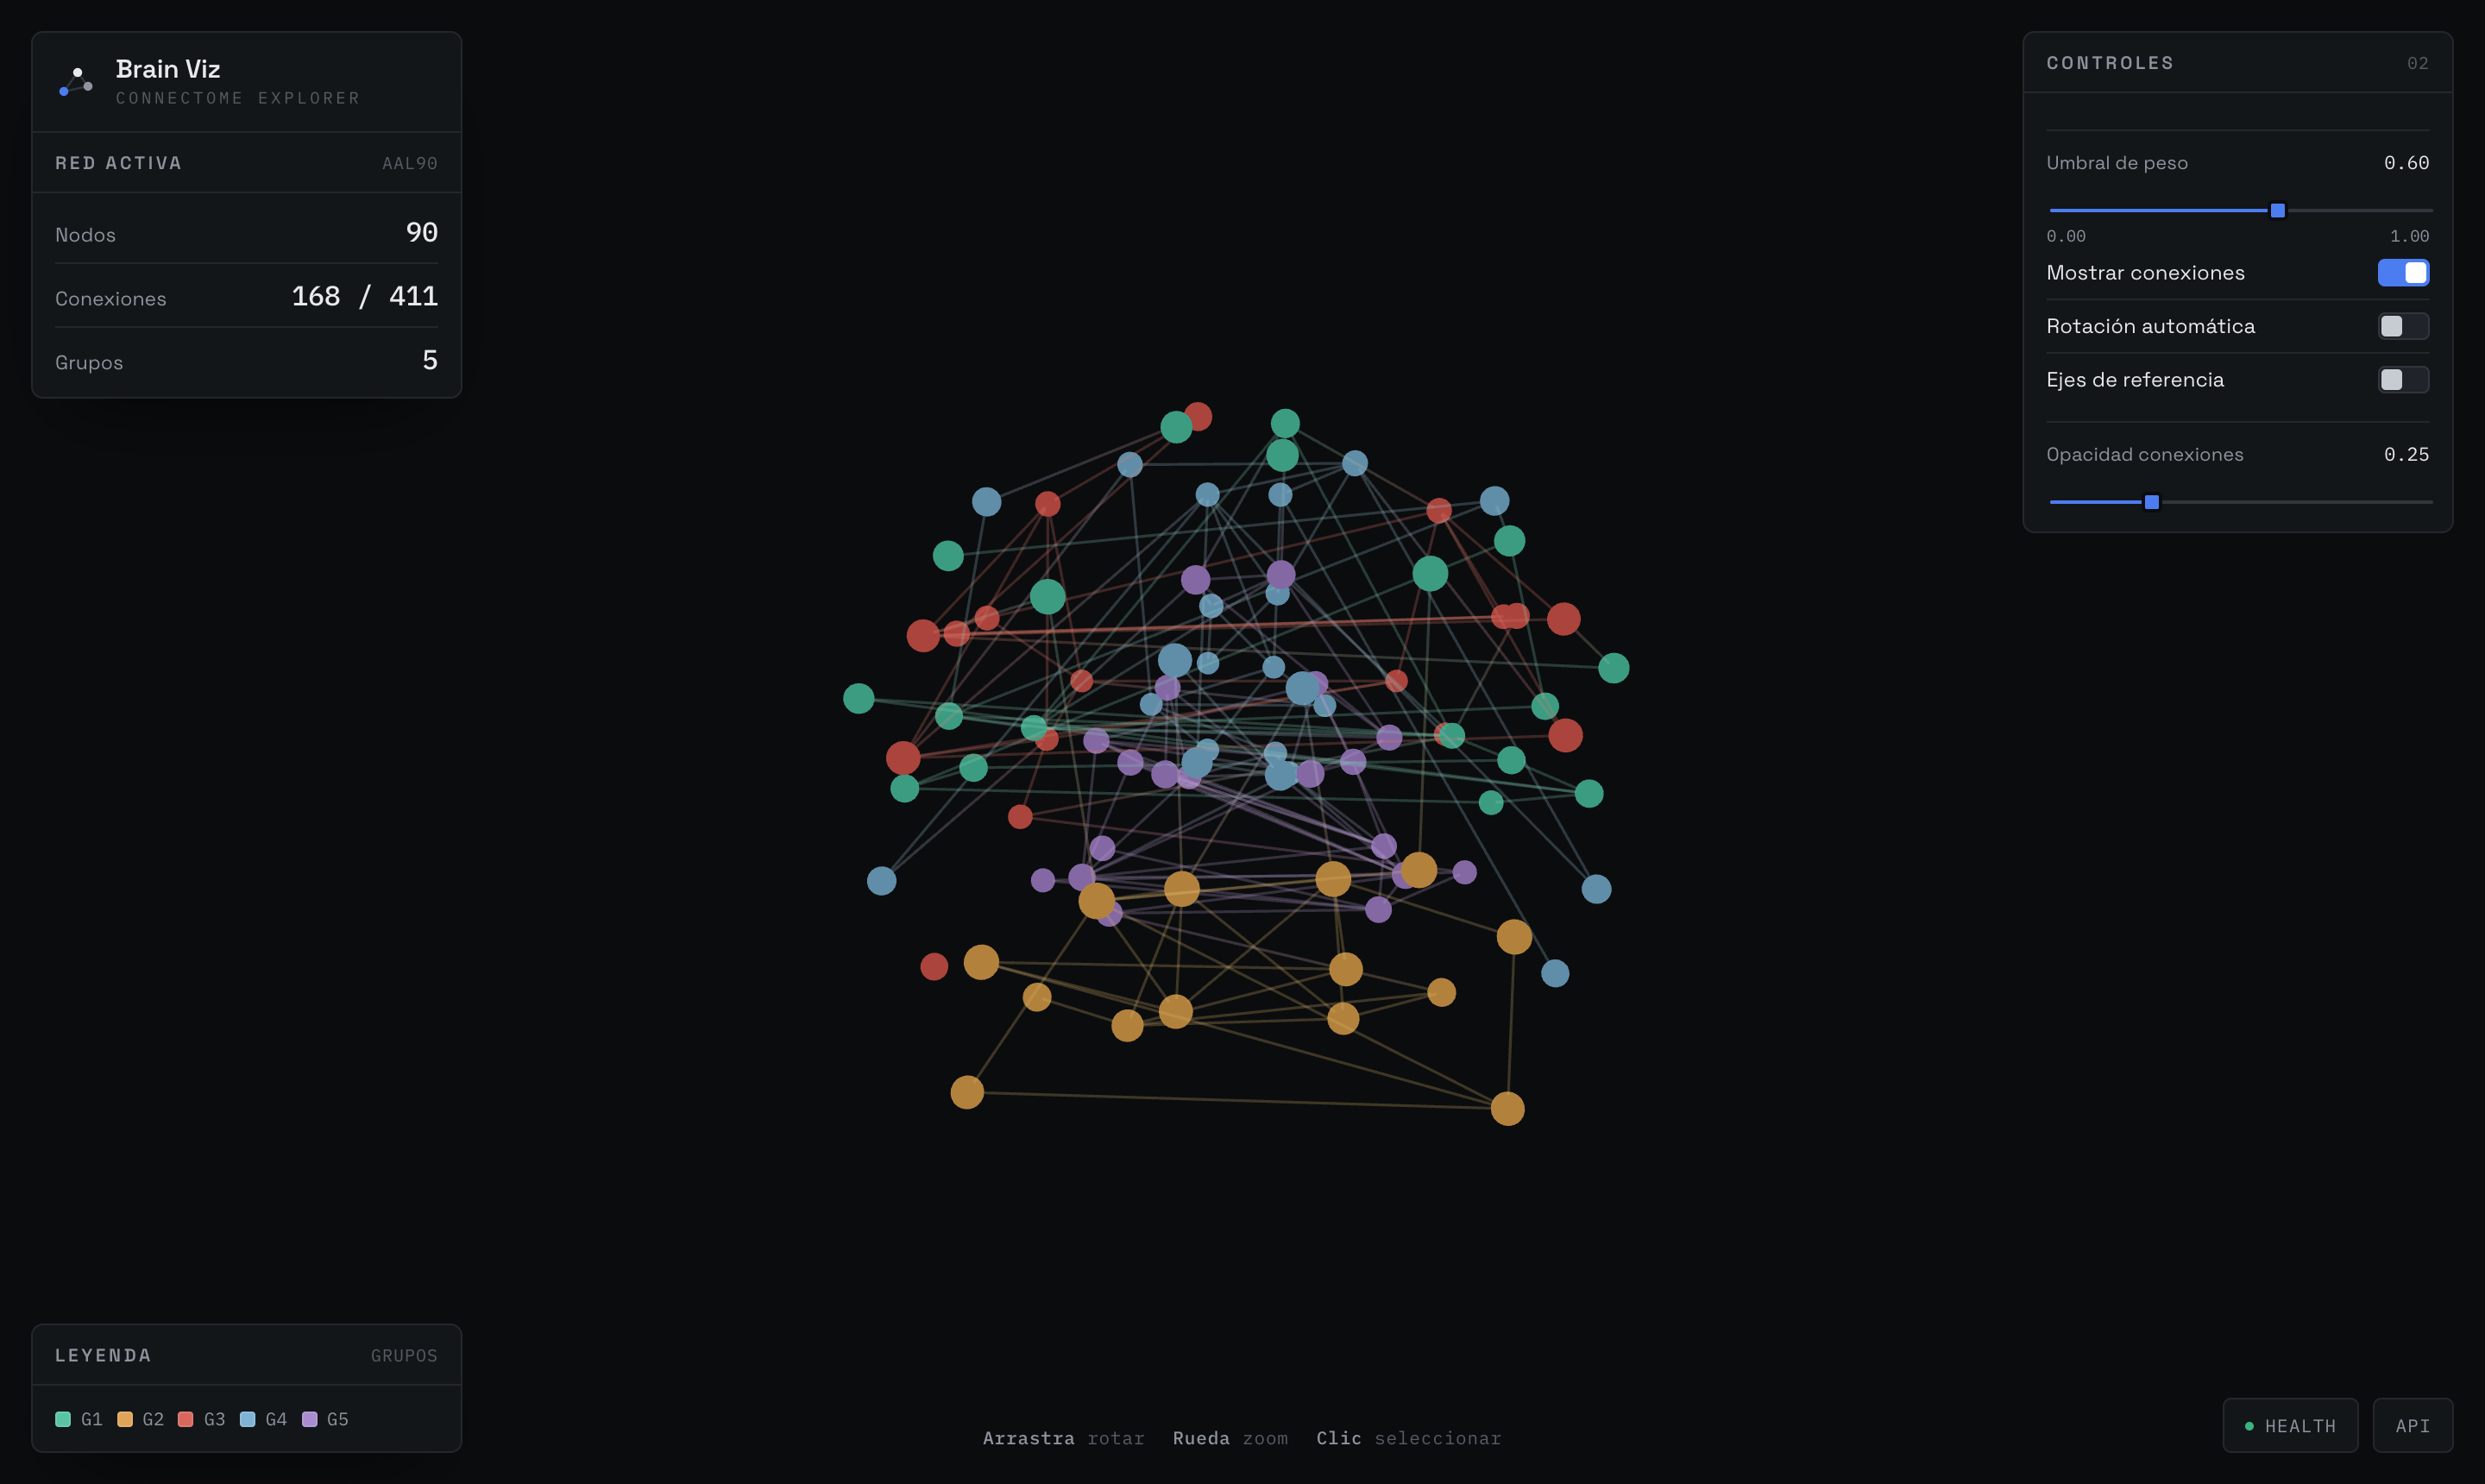
\includegraphics[width=0.86\textwidth]{imagenes/app_s2_umbral_alto}
	\caption{Filtrado por umbral (RF 5). Arriba: umbral 0,00, se muestran las 411 conexiones de la
	red. Abajo: umbral 0,60, quedan 168 conexiones y la estructura de la red se aprecia con mayor
	claridad. El contador del panel de estadísticas refleja en ambos casos la relación
	\textit{visibles / totales}.}
	\label{fig:s2-umbral}
\end{figure}

\begin{figure}[H]
	\centering
	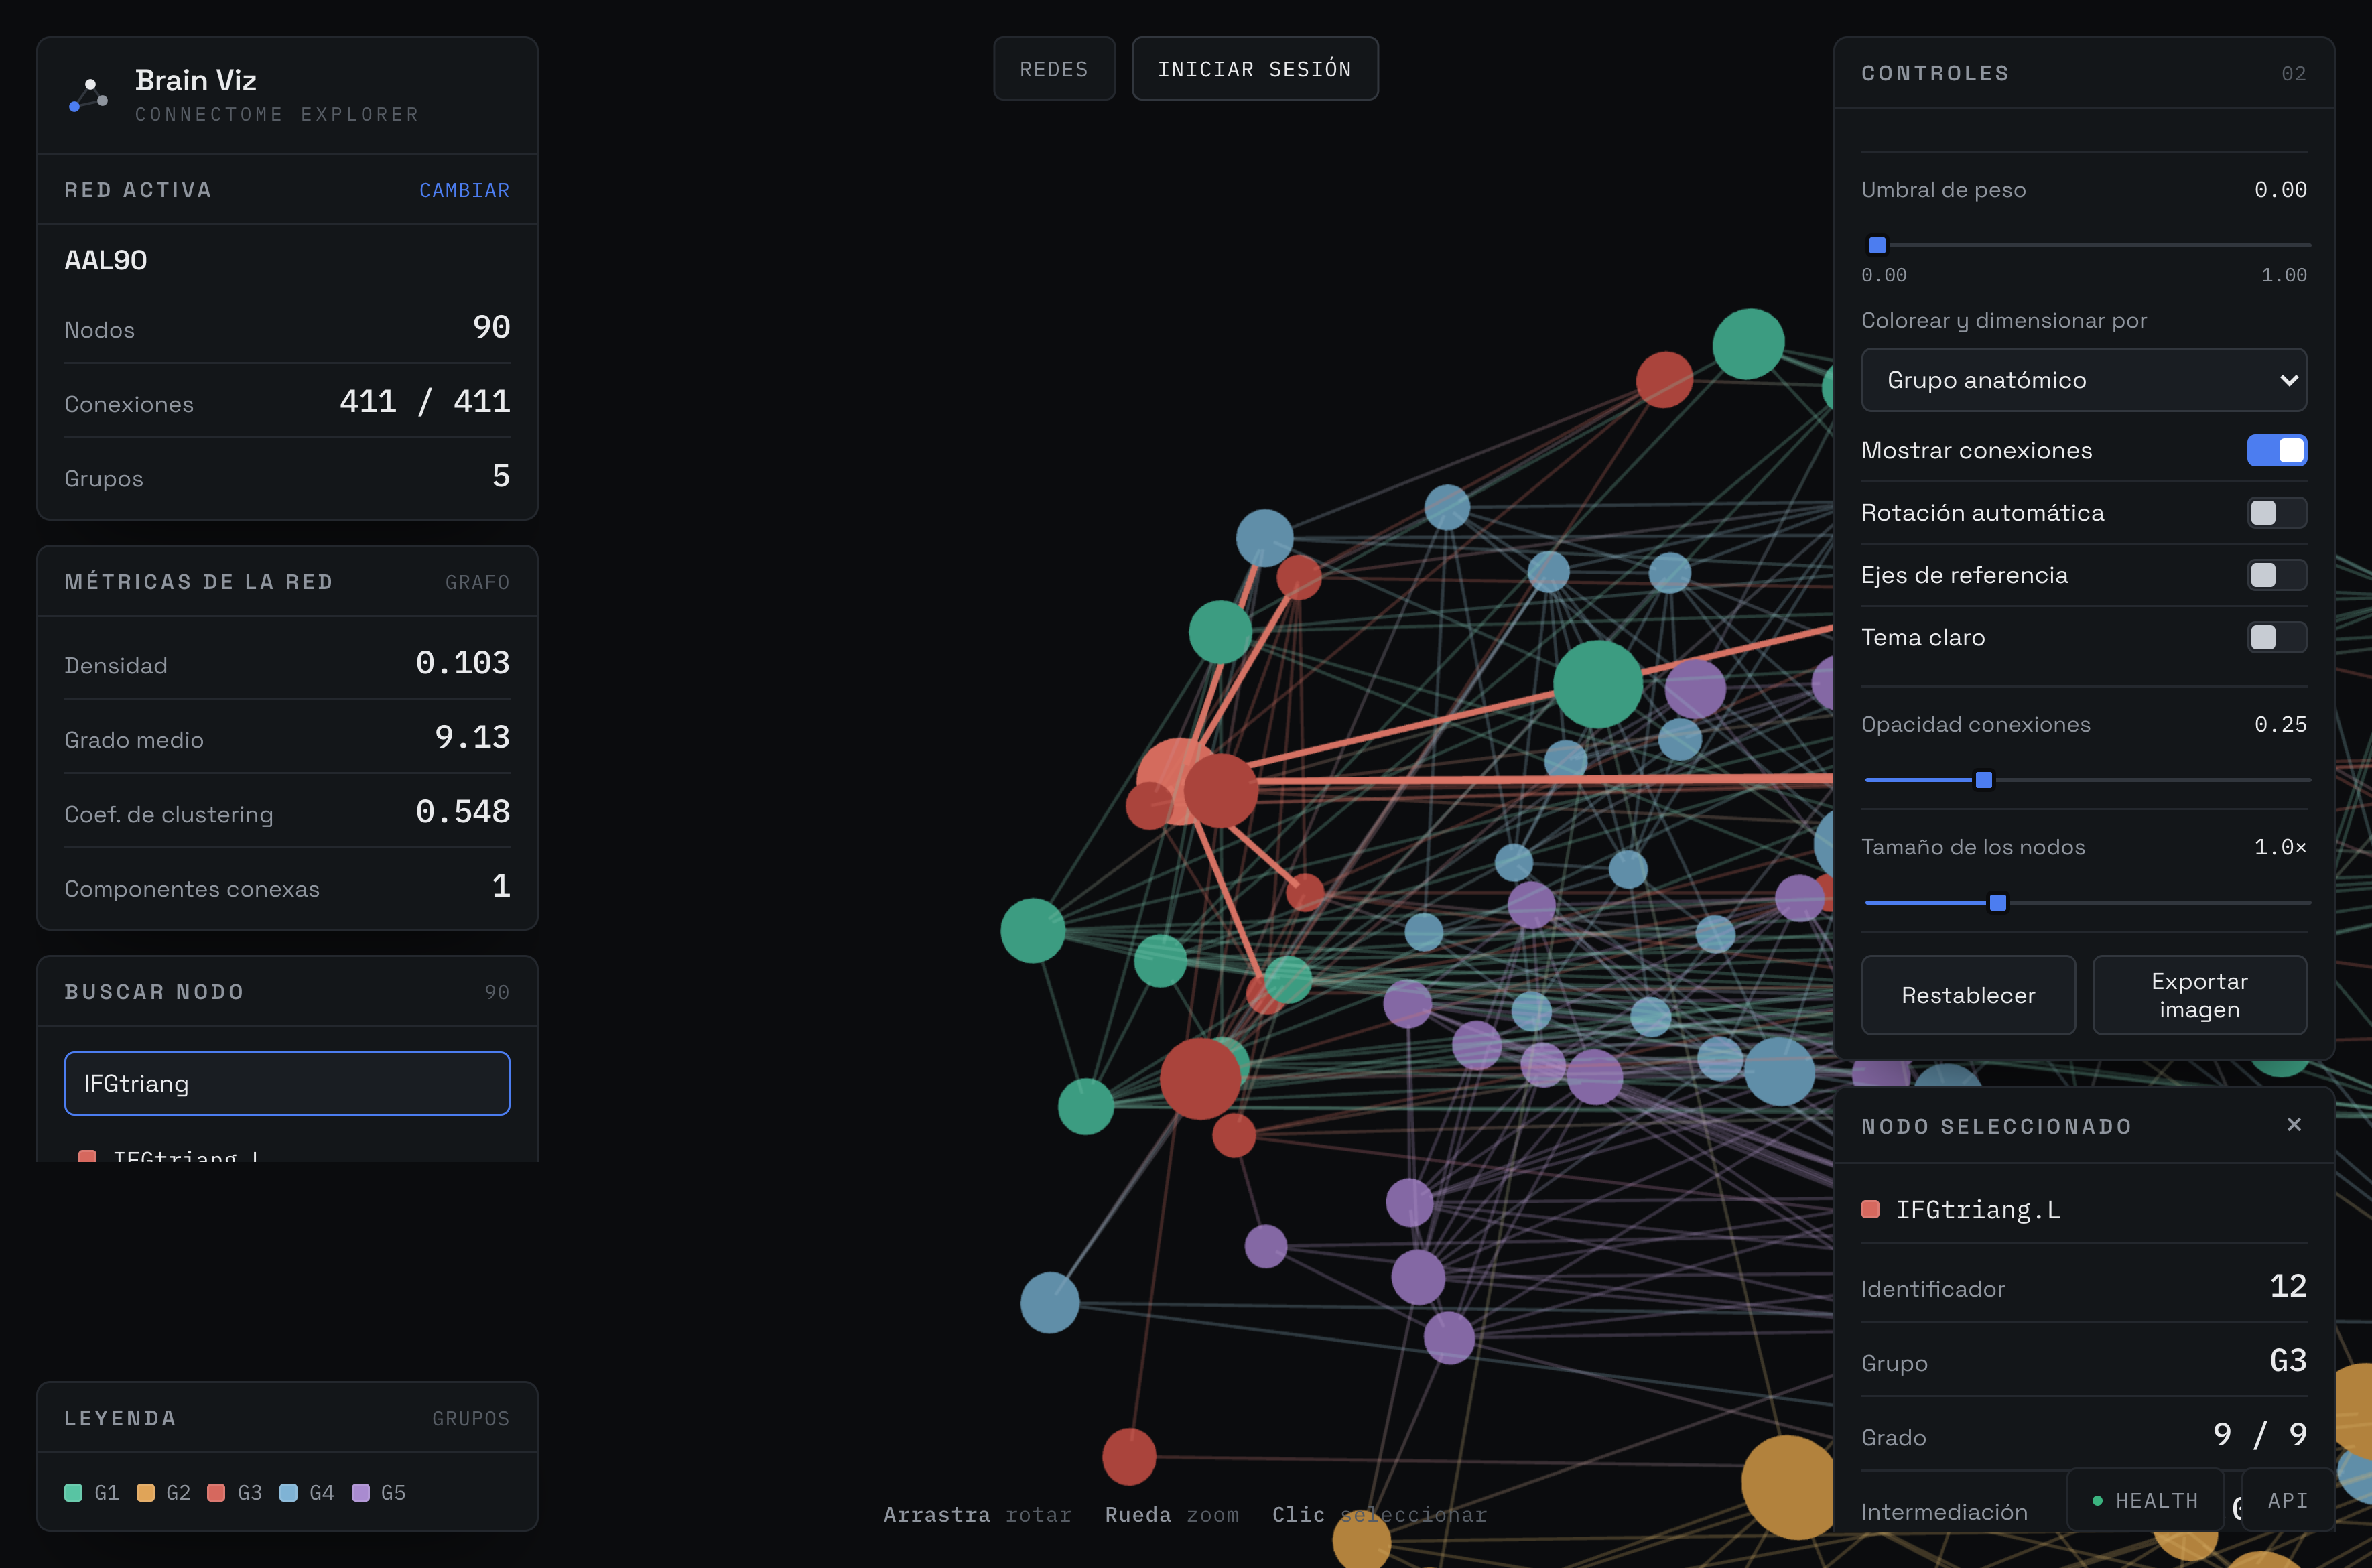
\includegraphics[width=\textwidth]{imagenes/app_s2_seleccion}
	\caption{Selección e inspección de un nodo (RF 6): la región \texttt{PoCG.L} aparece resaltada en la
	escena y el panel lateral muestra su identificador, grupo, grado y coordenadas.}
	\label{fig:s2-seleccion}
\end{figure}

\subsection{Pruebas}

Siguiendo la estrategia establecida en el \textit{sprint} anterior, las pruebas combinan caja blanca,
caja negra y validación.

\subsubsection*{Pruebas de caja blanca (unitarias)}

Se ha comprobado sobre el módulo de parseo que: el número de aristas devueltas coincide con el de
pares con peso no nulo de la matriz (411 en la red de ejemplo); la lista de aristas está efectivamente
ordenada de mayor a menor peso; el rango de pesos declarado en los metadatos coincide con el mínimo y
el máximo reales; y se cumple la identidad $\sum_i \text{grado}(i) = 2 \cdot |A|$, que verifica la
coherencia entre los grados calculados y el número de aristas. También se han probado los casos de
error: ficheros inexistentes, matriz no cuadrada y matriz cuyas dimensiones no coinciden con el número
de nodos.

\subsubsection*{Pruebas de caja negra (de integración)}

Se ha verificado que la respuesta de la API respeta el contrato ampliado, comprobando que cada nodo
incluye el atributo \texttt{degree} y que los metadatos incorporan \texttt{min\_weight} y
\texttt{max\_weight}. Sobre la aplicación en ejecución se ha contrastado que el contador de aristas
visibles que muestra la interfaz coincide, para distintos umbrales, con el número de aristas que
superan ese peso según los datos servidos por la API.

\subsubsection*{Pruebas de validación (de aceptación)}

La tabla~\ref{tab:pruebas-s2} recoge las pruebas de validación de los requisitos de este
\textit{sprint} y su resultado.

\begin{table}[H]
	\centering
	\caption{Pruebas de validación del Sprint 2.}
	\label{tab:pruebas-s2}
	\small
	\begin{tabularx}{\textwidth}{>{\raggedright\arraybackslash}p{1.5cm} >{\raggedright\arraybackslash}X >{\raggedright\arraybackslash}X >{\centering\arraybackslash}p{1.6cm}}
		\toprule
		\textbf{Prueba} & \textbf{Descripción} & \textbf{Resultado esperado} & \textbf{Estado} \\
		\midrule
		P-06 (RF 5) & Mover el control de umbral y observar la escena. &
			Las conexiones por debajo del umbral desaparecen de forma inmediata, sin esperas
			perceptibles. & Correcto \\
		\addlinespace
		P-07 (RF 5) & Comprobar el contador \textit{visibles / totales}. &
			Con umbral 0,50 se muestran 209 de 411 conexiones, cifra que coincide con el recuento sobre
			los datos de la API. & Correcto \\
		\addlinespace
		P-08 (RF 6) & Hacer clic sobre un nodo. &
			El nodo queda resaltado y se abre el panel con su etiqueta, identificador, grupo, grado y
			coordenadas. & Correcto \\
		\addlinespace
		P-09 (RF 6) & Contrastar el grado mostrado con el de la red. &
			El grado del panel coincide con el número de conexiones del nodo en los datos servidos. &
			Correcto \\
		\addlinespace
		P-10 (RF 6) & Hacer clic fuera de un nodo y pulsar el botón de cierre. &
			En ambos casos el nodo se deselecciona y el panel se cierra. & Correcto \\
		\addlinespace
		P-11 (RF 7) & Comprobar el coloreado por grupo y la leyenda. &
			Los nodos de un mismo grupo comparten color y la leyenda recoge los 5 grupos presentes. &
			Correcto \\
		\bottomrule
	\end{tabularx}
\end{table}

\subsubsection*{Pruebas de rendimiento (RNF 1)}

Una vez implementada la interacción, se ha abordado la comprobación del requisito no funcional de
fluidez [RNF 1]. Para poder evaluar el comportamiento con redes mayores que la de ejemplo, se ha
generado además una \textbf{red sintética de 500 nodos y 12.470 aristas} ---unas treinta veces más
conexiones que AAL90---, próxima al tamaño de referencia que fija el requisito. La medición se ha
realizado con un navegador controlado de forma automatizada, activando la rotación automática para
forzar un renderizado continuo (caso más desfavorable) y midiendo los intervalos entre fotogramas.
La tabla~\ref{tab:rendimiento} recoge los resultados.

\begin{table}[H]
	\centering
	\caption{Medición del rendimiento gráfico.}
	\label{tab:rendimiento}
	\small
	\begin{tabularx}{\textwidth}{>{\raggedright\arraybackslash}X >{\centering\arraybackslash}p{2.2cm} >{\centering\arraybackslash}p{2.2cm} >{\centering\arraybackslash}p{2.6cm}}
		\toprule
		\textbf{Red} & \textbf{Nodos} & \textbf{Aristas} & \textbf{Fotogramas/s} \\
		\midrule
		AAL90 (red de ejemplo)      & 90  & 411    & 30 \\
		Red sintética de prueba     & 500 & 12.470 & 30 \\
		\addlinespace
		\textit{Página vacía (referencia del entorno)} & --- & --- & \textit{30} \\
		\bottomrule
	\end{tabularx}
\end{table}

La interpretación de estos datos exige una precaución importante: al medir una \textbf{página vacía}
en el mismo entorno se obtiene también 30~fotogramas por segundo, lo que revela que es el propio
entorno de medida automatizado el que limita la tasa a ese valor. Por tanto, la medición
\emph{no permite verificar el objetivo de 60~FPS}, ya que ese techo no procede de la aplicación.

Lo que sí puede afirmarse es que la aplicación \textbf{sostiene el máximo que permite el entorno en
ambos casos}: multiplicar por treinta el número de aristas no produce ninguna degradación medible,
lo que indica que el renderizado no constituye un cuello de botella en el rango de tamaños
evaluado. Este resultado es coherente con la estrategia de diseño adoptada, que mantiene una única
geometría para todas las aristas y evita reconstruirla al filtrar. La verificación formal del
objetivo de $\geq 60$~FPS queda pendiente de realizarse con el perfilador de rendimiento de un
navegador de escritorio, y su resultado ---se alcance o no el objetivo--- se documentará en la
memoria final.

\subsubsection*{Errores detectados y corregidos}

Durante las pruebas de este \textit{sprint} se detectaron los siguientes errores:

\begin{itemize}
	\item \textbf{Grado incorrecto por aristas de peso nulo.} La primera versión calculaba el grado
		sobre el grafo construido directamente desde la matriz de adyacencia. Al comprobar la identidad
		$\sum_i \text{grado}(i) = 2 \cdot |A|$ se observó que no se cumplía: la librería creaba una
		arista por cada celda de la matriz, incluidas las de peso cero, de modo que todos los nodos
		presentaban el mismo grado (89, todos conectados con todos). Se corrigió eliminando del grafo
		las aristas de peso nulo antes de calcular los grados.
	\item \textbf{La deselección no cerraba el panel.} Durante la prueba automatizada, un clic en una
		zona aparentemente vacía no cerraba el panel de información. Al investigarlo se comprobó que el
		clic impactaba en realidad sobre el panel de la leyenda, superpuesto al lienzo, y que la
		deselección sí funcionaba al pulsar sobre una región libre de la escena. El error estaba en la
		prueba y no en la aplicación, pero el caso se documenta porque obligó a delimitar con precisión
		las zonas interactivas de la interfaz.
\end{itemize}

\subsubsection*{Validación por parte del cliente}

Al igual que en el \textit{sprint} anterior, la validación final corresponde al director del proyecto.
Para hacerla posible, la aplicación se ha \textbf{desplegado en un servidor accesible desde Internet},
de modo que tanto el director como, más adelante, los miembros del tribunal puedan probarla sin
instalar nada.

El despliegue emplea una \textbf{imagen de producción} distinta de la utilizada en desarrollo: en
lugar de dos servicios comunicados por un \textit{proxy} interno, se genera un único contenedor en el
que la interfaz de React se compila a ficheros estáticos y es servida por el propio \textit{backend}
mediante un servidor WSGI de producción. Esta decisión simplifica el despliegue, elimina la
dependencia de la red interna de contenedores y evita ejecutar servidores de desarrollo ---o el modo
de depuración--- en una dirección pública. El procedimiento completo se detalla en el manual de
instalación.
% NOTA: insertar aquí la URL pública del despliegue.


	\chapter{Manual de instalación}

En este capítulo se detalla el procedimiento para instalar y ejecutar la aplicación. Gracias al uso
de contenedores, el despliegue es reproducible y no requiere instalar manualmente las dependencias
de Python ni de Node.js: basta con disponer de Docker.

El proyecto contempla dos formas de ejecución, pensadas para propósitos distintos. La
\textbf{ejecución en local} (secciones~\ref{sec:requisitos} y~\ref{sec:lanzamiento}) levanta los dos
servicios por separado con Docker Compose y recarga en caliente, que es lo adecuado durante el
desarrollo. El \textbf{despliegue en un servidor público} (sección~\ref{sec:despliegue}) emplea, en
cambio, una única imagen autocontenida pensada para producción.

\section{Requisitos previos}
\label{sec:requisitos}

Para ejecutar la aplicación es necesario contar con:

\begin{itemize}
	\item \textbf{Docker}~\cite{docker} y \textbf{Docker Compose} instalados y en ejecución. En Windows y macOS
		se recomienda instalar \textit{Docker Desktop}; en Linux, el motor de Docker junto con el
		\textit{plugin} de Compose.
	\item Los \textbf{ficheros de datos} del atlas de ejemplo (\texttt{AAL90.node} y
		\texttt{AAL90.edge}) ubicados en el directorio \texttt{backend/data/} del proyecto.
	\item Un \textbf{navegador moderno} con soporte de WebGL 2.0 (Chrome, Firefox o Edge).
\end{itemize}

Puede comprobarse que Docker está correctamente instalado con:

\begin{verbatim}
docker --version
docker compose version
\end{verbatim}

\section{Instalación y lanzamiento en local}
\label{sec:lanzamiento}

Una vez clonado o descargado el repositorio, se accede a su directorio raíz y se construyen y
levantan los contenedores.

\subsection{Alternativa 1: recomendada}

Se emplea el \textit{script} auxiliar incluido en el proyecto, que levanta los servicios y muestra
por consola los puertos asignados automáticamente:

\begin{verbatim}
./up-brain-viz.sh
\end{verbatim}

\subsection{Alternativa 2}

De forma equivalente, se pueden construir y levantar los contenedores directamente con Docker
Compose:

\begin{verbatim}
docker compose up --build
\end{verbatim}

\subsection{Post-ejecución y resumen}

Los servicios de \textit{backend} y \textit{frontend} exponen sus puertos internos (5000 y 5173,
respectivamente) en puertos del anfitrión asignados automáticamente, evitando conflictos con otros
procesos. Para conocer los puertos publicados se ejecuta:

\begin{verbatim}
docker compose ps
\end{verbatim}

A partir de la columna de puertos publicados se obtiene la dirección de acceso; por ejemplo, el
frontend estará disponible en \texttt{http://localhost:<puerto>}. Para detener la aplicación:

\begin{verbatim}
docker compose down
\end{verbatim}

\subsection{Consideraciones}

\begin{itemize}
	\item El navegador se comunica únicamente con el \textit{frontend}; las peticiones a
		\texttt{/api} y \texttt{/health} se redirigen internamente al \textit{backend} dentro de la
		red de contenedores.
	\item El entorno está configurado para desarrollo con recarga en caliente
		(\textit{hot-reload}): los cambios en el código fuente se reflejan sin reconstruir la imagen.
	\item El \textit{script} \texttt{get-docker.sh} incluido en el repositorio es un instalador de
		Docker para Linux; en macOS y Windows debe usarse Docker Desktop.
\end{itemize}

\section{Despliegue en un servidor público}
\label{sec:despliegue}

Además de la ejecución en local, la aplicación se despliega en un servidor accesible desde Internet
para que el director del proyecto pueda validar cada \textit{sprint} y para que el tribunal pueda
probarla sin necesidad de instalar nada.

\subsection{Imagen de producción}

El modo de desarrollo descrito en la sección anterior no es adecuado para un servidor público por dos
motivos: emplea servidores de desarrollo ---tanto el de Vite como el integrado de Flask, que no están
pensados para producción y no deben ejecutarse con el modo de depuración activo en una dirección
pública--- y reparte la aplicación en dos servicios que se comunican mediante un nombre interno de la
red de Docker Compose, inexistente fuera de ella.

Por ello se ha añadido un \texttt{Dockerfile} en la raíz del proyecto que genera una \textbf{imagen
única de producción} en dos etapas:

\begin{enumerate}
	\item En la primera etapa se compila la aplicación de React, obteniendo un conjunto de ficheros
		estáticos optimizados.
	\item En la segunda, esos ficheros se copian a la imagen de Python, donde el propio servidor sirve
		tanto la interfaz como la API.
\end{enumerate}

De este modo todo el sistema queda en un solo contenedor, desaparece la necesidad de un \textit{proxy}
entre servicios y la imagen puede desplegarse en cualquier plataforma que admita contenedores. La
aplicación se ejecuta con \textbf{gunicorn}, un servidor WSGI de producción, escuchando en todas las
interfaces y en el puerto que indique la variable de entorno \texttt{PORT}, tal y como esperan las
plataformas de despliegue habituales. La imagen puede construirse y probarse en local con:

\begin{verbatim}
docker build -t brain-viz:prod .
docker run -p 8080:8080 brain-viz:prod
\end{verbatim}

\subsection{Publicación}

El repositorio incluye un fichero \texttt{render.yaml} que describe el servicio, de forma que la
plataforma de despliegue detecta la configuración automáticamente a partir del repositorio: tipo de
servicio, ruta del \texttt{Dockerfile}, región y ruta de comprobación de estado (\texttt{/health}).
Cada nueva versión publicada en la rama principal del repositorio desencadena un nuevo despliegue.

% NOTA: insertar aquí la URL pública una vez completado el despliegue.

\subsection{Consideraciones del entorno gratuito}

El servicio se aloja en un plan gratuito, lo que conlleva una limitación que conviene conocer: la
instancia se suspende tras un periodo de inactividad, de modo que la primera petición tras ese
periodo puede tardar aproximadamente un minuto mientras el servicio se reactiva; las siguientes se
atienden con normalidad. Para reducir este efecto durante los periodos de evaluación se emplea un
servicio externo de comprobación periódica que consulta el \textit{endpoint} \texttt{/health} a
intervalos regulares, manteniendo la instancia activa.
  % Cap. 5 - Manual de instalación
	\chapter{Manual de usuario}

Este capítulo explica cómo utilizar la aplicación una vez desplegada. Dado que el sistema cuenta con
un único rol de usuario, el manual se organiza en función de las tareas que este puede realizar, en
lugar de por perfiles. El contenido se irá ampliando a medida que se completen los sucesivos
\textit{sprints}.

\section{Acceso y visión general}

Al abrir la aplicación en el navegador se muestra una pantalla de acceso de carácter presentacional.
Tras acceder, se presenta la red cerebral de ejemplo (atlas AAL90) ya renderizada en el lienzo 3D,
junto con los paneles de información y control superpuestos.

% NOTA: incluir captura de la pantalla de acceso y de la vista general.

\section{Navegación por la escena 3D}

El usuario puede explorar la red mediante los controles de cámara:

\begin{itemize}
	\item \textbf{Rotar (orbitar):} arrastrar con el botón izquierdo del ratón.
	\item \textbf{Zoom:} rueda del ratón o gesto de pellizco en dispositivos táctiles.
	\item \textbf{Desplazar (paneo):} arrastrar con el botón derecho o con dos dedos.
\end{itemize}

\section{Interpretación de la visualización}

Cada nodo representa una región cerebral situada en sus coordenadas anatómicas, y su color indica el
grupo o lóbulo al que pertenece, según la leyenda mostrada en la interfaz. Las líneas entre nodos
representan las conexiones de la red. El panel de estadísticas muestra el número de nodos,
conexiones y grupos de la red activa.

% NOTA: a medida que avancen los sprints, documentar aquí el filtrado por umbral (RF 5), la
% selección e inspección de nodos (RF 6, RF 6.1), la consulta de métricas (RF 8), la búsqueda
% (RF 10), y las funciones de investigador/administrador: registro (RF 13), carga de datasets
% propios (RF 14), gestión de datasets (RF 15) y exportación (RF 12, RF 16).
      % Cap. 6 - Manual de usuario
	\chapter{Conclusiones}

% NOTA: capítulo a completar al finalizar el desarrollo. Debe recoger una valoración del trabajo
% realizado, el grado de cumplimiento de los objetivos planteados en la introducción y una
% reflexión personal, además de las líneas de mejora y trabajo futuro.

\section{Experiencia personal}

% Reflexión sobre el proceso de desarrollo: aprendizajes técnicos (stack web moderno, visualización
% 3D con WebGL, contenedores), dificultades encontradas y su resolución, y valoración global del
% cumplimiento de los objetivos.

\section{Propuesta de mejoras}

Entre las principales líneas de trabajo futuro se contemplan:

\begin{itemize}
	\item Optimización del rendimiento para grafos de gran tamaño (más de 1000 nodos) mediante
		técnicas como el nivel de detalle (LOD) o el uso de \textit{web workers} para los cálculos
		más pesados.
	\item Incorporación de análisis de red más avanzados, como la detección de comunidades o el
		cálculo de caminos mínimos entre regiones.
	\item Soporte para más atlas y formatos de datos públicos.
	\item Autenticación real y persistencia de configuraciones de usuario.
\end{itemize}
        % Cap. 7 - Conclusiones

	\newpage
	\bibliography{bibliografia}
	\bibliographystyle{plain}
	
\end{document}

